%definira klasu dokumenta 
\documentclass[12pt]{report} 

%prostor izmedu naredbi \documentclass i \begin{document} se zove uvod. U njemu se nalaze naredbe koje se odnose na cijeli dokument

%osnovni LaTex ne može riješiti sve probleme, pa se koriste različiti paketi koji olakšavaju izradu željenog dokumenta
\usepackage[croatian]{babel} 
\usepackage{amssymb}
\usepackage{amsmath}
\usepackage{txfonts}
\usepackage{mathdots}
\usepackage{titlesec}
\usepackage{array}
\usepackage{lastpage}
\usepackage{etoolbox}
\usepackage{tabularray}
\usepackage{color, colortbl}
\usepackage{adjustbox}
\usepackage{geometry}
\usepackage[classicReIm]{kpfonts}
\usepackage{hyperref}
\usepackage{fancyhdr}

\usepackage{float}
\usepackage{setspace}
\restylefloat{table}


\patchcmd{\chapter}{\thispagestyle{plain}}{\thispagestyle{fancy}}{}{} %redefiniranje stila stranice u paketu fancyhdr

%oblik naslova poglavlja
\titleformat{\chapter}{\normalfont\huge\bfseries}{\thechapter.}{20pt}{\Huge}
\titlespacing{\chapter}{0pt}{0pt}{40pt}


\linespread{1.3} %razmak između redaka

\geometry{a4paper, left=1in, top=1in,}  %oblik stranice

\hypersetup{ colorlinks, citecolor=black, filecolor=black, linkcolor=black,	urlcolor=black }   %izgled poveznice


%prored smanjen između redaka u nabrajanjima i popisima
\newenvironment{packed_enum}{
	\begin{enumerate}
		\setlength{\itemsep}{0pt}
		\setlength{\parskip}{0pt}
		\setlength{\parsep}{0pt}
	}{\end{enumerate}}

\newenvironment{packed_item}{
	\begin{itemize}
		\setlength{\itemsep}{0pt}
		\setlength{\parskip}{0pt}
		\setlength{\parsep}{0pt}
	}{\end{itemize}}




%boja za privatni i udaljeni kljuc u tablicama
\definecolor{LightBlue}{rgb}{0.9,0.9,1}
\definecolor{LightGreen}{rgb}{0.9,1,0.9}

%Promjena teksta za dugačke tablice
\DefTblrTemplate{contfoot-text}{normal}{Nastavljeno na idućoj stranici}
\SetTblrTemplate{contfoot-text}{normal}
\DefTblrTemplate{conthead-text}{normal}{(Nastavljeno)}
\SetTblrTemplate{conthead-text}{normal}
\DefTblrTemplate{middlehead,lasthead}{normal}{Nastavljeno od prethodne stranice}
\SetTblrTemplate{middlehead,lasthead}{normal}

%podesavanje zaglavlja i podnožja

\pagestyle{fancy}
\lhead{Programsko inženjerstvo}
\rhead{$<$Projektni zadatak$>$}
\lfoot{$<$Naziv grupe$>$}
\cfoot{stranica \thepage/\pageref{LastPage}}
\rfoot{\today}
\renewcommand{\headrulewidth}{0.2pt}
\renewcommand{\footrulewidth}{0.2pt}


\begin{document} 
	
	
	
	\begin{titlepage}
		\begin{center}
			\vspace*{\stretch{1.0}} %u kombinaciji s ostalim \vspace naredbama definira razmak između redaka teksta
			\LARGE Programsko inženjerstvo\\
			\large Ak. god. 2020./2021.\\
			
			\vspace*{\stretch{3.0}}
			
			\huge $<$Naziv projekta$>$\\
			\Large Dokumentacija, Rev. \textit{$<$1 ili 2$>$}\\
			
			\vspace*{\stretch{12.0}}
			\normalsize
			Grupa: \textit{$<$Naziv grupe$>$}\\
			Voditelj: \textit{$<$Ime i prezime voditelja$>$}\\
			
			
			\vspace*{\stretch{1.0}}
			Datum predaje: \textit{$<$dan$>$. $<$mjesec$>$. $<$godina$>$.}\\
	
			\vspace*{\stretch{4.0}}
			
			Nastavnik: \textit{$<$Ime i prezime nastavnika zaduženog za vašu grupu$>$}\\
		
		\end{center}

	
	\end{titlepage}

	
	\tableofcontents


	\chapter{Dnevnik promjena dokumentacije}
		
		\textbf{\textit{Kontinuirano osvježavanje}}\\
				
		
		\begin{longtblr}[
				label=none
			]{
				width = \textwidth, 
				colspec={|X[2]|X[13]|X[3]|X[3]|}, 
				rowhead = 1
			}
			\hline
			\textbf{Rev.}	& \textbf{Opis promjene/dodatka} & \textbf{Autori} & \textbf{Datum}\\[3pt] \hline
			0.1 & Napravljen predložak.	& * & 22.08.2013. 		\\[3pt] \hline 
			0.2	& Dopisane upute za povijest dokumentacije.\newline Dodane reference. & * & 24.08.2013. 	\\[3pt] \hline 
			0.5 & Dodan \textit{Use Case} dijagram i jedan sekvencijski dijagram, funkcionalni i nefunkcionalni zahtjevi i dodatak A & * & 25.08.2013. \\[3pt] \hline 
			0.6 & Arhitektura i dizajn sustava, algoritmi i strukture podataka & * & 26.08.2013. \\[3pt] \hline 
			0.8 & Povijest rada i trenutni status implementacije,\newline Zaključci i plan daljnjeg rada & * & 28.08.2013. \\[3pt] \hline 
			0.9 & Opisi obrazaca uporabe & * & 07.09.2013. \\[3pt] \hline 
			0.10 & Preveden uvod & * & 08.09.2013. \\[3pt] \hline 
			0.11 & Sekvencijski dijagrami & * & 09.09.2013. \\[3pt] \hline 
			0.12.1 & Započeo dijagrame razreda & * & 10.09.2013. \\[3pt] \hline 
			0.12.2 & Nastavak dijagrama razreda & * & 11.09.2013. \\[3pt] \hline 
			\textbf{1.0} & Verzija samo s bitnim dijelovima za 1. ciklus & * & 11.09.2013. \\[3pt] \hline 
			1.1 & Uređivanje teksta -- funkcionalni i nefunkcionalni zahtjevi & * \newline * & 14.09.2013. \\[3pt] \hline 
			1.2 & Manje izmjene:Timer - Brojilo vremena & * & 15.09.2013. \\[3pt] \hline 
			1.3 & Popravljeni dijagrami obrazaca uporabe & * & 15.09.2013. \\[3pt] \hline 
			1.5 & Generalna revizija strukture dokumenta & * & 19.09.2013. \\[3pt] \hline 
			1.5.1 & Manja revizija (dijagram razmještaja) & * & 20.09.2013. \\[3pt] \hline 
			\textbf{2.0} & Konačni tekst predloška dokumentacije  & * & 28.09.2013. \\[3pt] \hline 
			&  &  & \\[3pt] \hline	
		\end{longtblr}
	
	
		\textit{Moraju postojati glavne revizije dokumenata 1.0 i 2.0 na kraju prvog i drugog ciklusa. Između tih revizija mogu postojati manje revizije već prema tome kako se dokument bude nadopunjavao. Očekuje se da nakon svake značajnije promjene (dodatka, izmjene, uklanjanja dijelova teksta i popratnih grafičkih sadržaja) dokumenta se to zabilježi kao revizija. Npr., revizije unutar prvog ciklusa će imati oznake 0.1, 0.2, …, 0.9, 0.10, 0.11.. sve do konačne revizije prvog ciklusa 1.0. U drugom ciklusu se nastavlja s revizijama 1.1, 1.2, itd.}
	\chapter{Opis projektnog zadatka}
		
%		\textbf{\textit{dio 1. revizije}}\\

	\section{Cilj i opis projekta na temelju dobivenog zadatka}	
	Cilj projekta je razviti web aplikaciju koja omogućuje dijeljenje recepata te tako pomaže korisnicima pri dijeljenju kulinarskih ideja, suradnji s drugim kreatorima recepata, organizaciji vlastite dijete i otkrivanju novih načina za pripremu jela. Tako korist od nje mogu imati profesionalni kuhari, nutricionisti, ali i kuhari amateri te osobe koje radi zdravstvenog stanja moraju prilagođavati dijetu. Novopridošlim korisnicima se prikazuju recepti sortirani od novijih prema starijima, što omogućuje da bez registracije imaju pregled kulinarskih trendova i odluče hoće li je nastaviti koristiti. Moguće se registrirati kao klijent, kuharski entuzijast ili nutricionist. Korisnik može administratorima poslati zahtjev za registraciju koji, jednom kad je odobren, dopušta korisniku da pretražuje profile i recepte na temelju dijete koju prate. Entuzijasti kreiraju recepte i kuharice, koje su skupovi recepata, dok nutricionisti kreiraju dijete koje nameću ograničenja na recepte. Korisnici neposredno prije kuhanja mogu unijeti prehrambeni artikl QR kodom ili izborom iz kataloga te tako filtrirati recepte u kojima se on nalazi. Tada se recepti sortiraju prema tome koliko dobro prate dijetu korisnika, odnosno koliko poštuju njena ograničenja. Korisnici također vide statistiku povijesti unosa nutritivnih vrijednosti. Što se implementacije tiče, aplikacija mora biti objektno orijentirana.

	\section{Potencijalna korist projekta}
	Osim očite koristi da korisnici među sobom dijele i objavljuju recepte i dijete, korist se može naći i u statistici unosa nutritivnih vrijednosti te vrstama recepata koju prate. Uzmimo u obzir da aplikacija \glqq zaživi\grqq, odnosno dostigne broj korisnika dovoljan da predstavlja državu ili neki njen dio. Tada bi vladajući mogli iskoristiti informaciju o tome što ljudi najviše jedu i subvencionirati domaće proizvođače tih proizvoda jer je njihova prodaja izglednija. S druge strane, mogli bi ciljati na raznolikost prehrane pa subvencionirati one koji proizvode hranu koja je u manjku. Profit tada nije tako izgledan kao u prvom slučaju, ali bi financijska motivacija navela proizvođače da se preusmjere te tako dođe do veće dostupnosti raznolike prehrane na tržištu. S obzirom da aplikacija vodi računa o preferencijama korisnika i dijetama koje odabiru, novi vlasnici restorana i drugih lokala koji poslužuju hranu bi mogli to iskoristiti da se specijaliziraju, odnosno nude proizvode u skladu s nekom dijetom. Kao što je naznačeno u rečenici prije, radilo bi se samo o preferencijama i dijetama, koje ne smatramo osobnim podatcima jer su to odabiri unutar aplikacije. Ljudi koji ne smiju konzumirati određene namirnice ili skupove namirnica radi zdravstvenog stanja ili uvjerenja ne mogu jesti u većini lokala. Podatci o dijetama i receptima koje korisnici vole omogućuju vlasnicima novih lokala da ponude takvim osobama obroke u obliku specijalnih menija ili pak specijaliziraju cijeli lokal za tu dijetu.

	\section{Slična, već postojeća rješenja}
	Kriteriji da rješenje smatramo sličnim:
	\begin{packed_item}
		\item Aplikacija/web mjesto mora biti forum, to jest mora imati mogućnost registriranja korisnika koji onda mogu raspravljati.
		\item Tema diskusije mora biti hrana.
		\item Mora postojati mogućnost filtriranja recepata prema više od jednog kriterija, ne nužno istovremeno.
	\end{packed_item}

		\subsection{kuhar.ba}
			\url{https://kuhar.ba} -- datum pristupa: 26.10.2023.
			Web mjesto na naslovnoj stranici ima mogućnost filtriranja recepata prema složenosti te kategorijama i grupama jela. Moguće se registrirati te potom dodavati recepte, komentirati ih te raspravljati na forumu. Recepti imaju fotografiju, popis sastojaka, detaljni opis koraka i oznake.
				\begin{figure}[H]
					\centering
					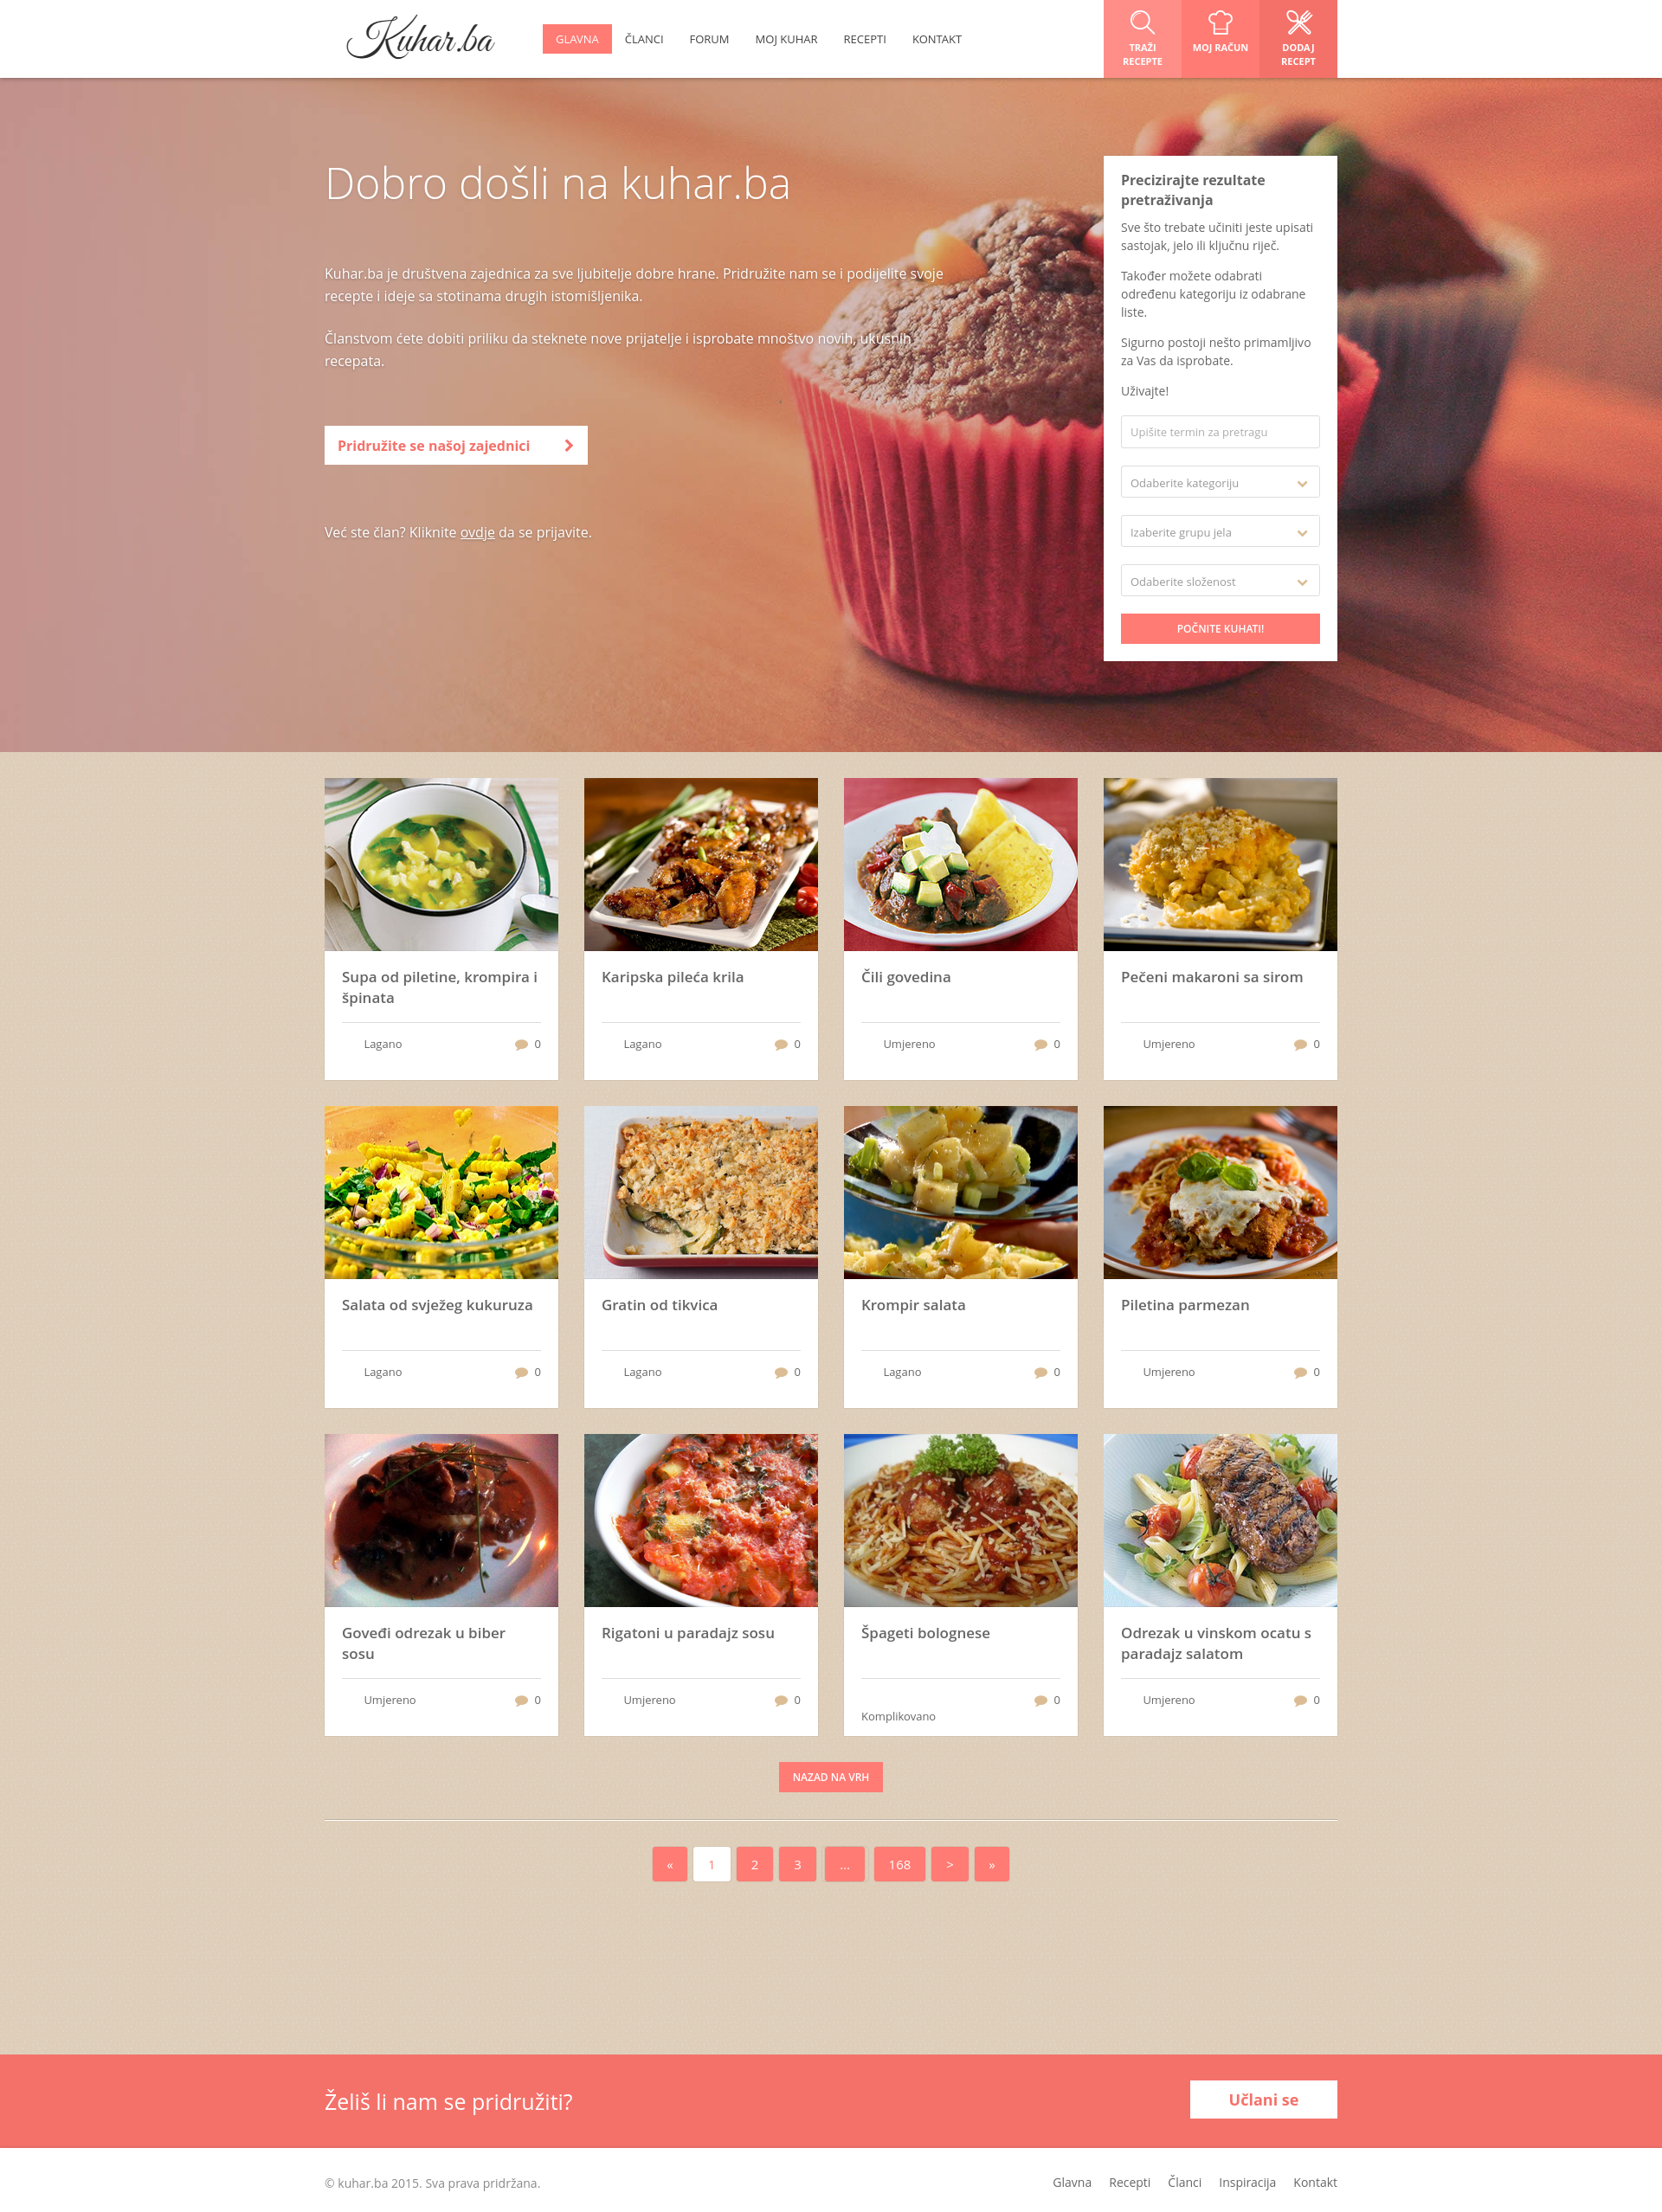
\includegraphics[scale=0.1]{slike/02-01-kuhar-ba.PNG}
					\caption{prednja strana web mjesta kuhar.ba}
					\label{fig:kuhar-ba-front}
				\end{figure} 
	

	\section{Skup korisnika koji bi mogao biti zainteresiran za ostvareno rješenje...}
		\subsection ... ako je aplikacija implementirana ovako
		\begin{packed_item}
			\item kulinarski entuzijasti
			\item nutricionisti
			\item klijenti
			\item[]\begin{packed_item}
				\item profesionalni kuhari
				\item kuhari amateri
				\item osobe kojima je potrebna specijalna dijeta radi zdravstvenih razloga ili uvjerenja
			\end{packed_item}
		\end{packed_item}
		
		\subsection ... ako je tematika aplikacije (u originalu kuhanje, to jest hrana) prilagođena ciljanim korisnicima
		\begin{packed_item}
			\item "uradi sam" majstori
			\item slikari
		\end{packed_item}
		Navedeni korisnici bi imali koristi od slične aplikacije. Općenitije, svaka zajednica ljudi za hobi ili zanimanje koje koristi algoritme, to jest radnje koje su podijeljene u niz koraka bi imalo koristi od slične aplikacije jer bi tako lakše razmjenjivali ideje i dolazili do inovacija u radu.

	\section{Mogućnost prilagodbe rješenja}
	Mana trenutnog rješenja je da ograničeno na objektno orijentirano pisanje jer to otežava skaliranje u budućnosti. Radi se o web (ili mobilnoj) aplikaciji koja treba imati sučelje koje je lako za razumjeti i koristi se u kuhinji, gdje, uz uobičajene laptope, mobitele i tablete, korisnici mogu imati i ostale pametne uređaje poput frižidera ili pećnica. Svi ti uređaji imaju web preglednik (ili operacijski sustav sličan Androidu ili nekoj konfiguraciji Linux-a) te su potencijalni klijenti. Što je više klijenata, baza podataka u pozadini je veća, a time i broj objekata, koji potiču problem upravljanja memorijom. Preporučeni programski jezici za poslužitelje, Java i Python uz Javascript, koji izvršavaju preglednici, svi redom koriste garbage collector. Činjenica je da taj proces šteti brzini rada aplikacije jer algoritam za "čišćenje" mora proći cijelu memoriju. Što više objekata, to više posla za taj algoritam pa stoga i veći period vremena koji sustav ili dijelovi sustava moraju provesti čekajući. Još k tomu niti dodavanje radne memorije ne pomaže jer to također algoritmu zadaje dodatan posao. Razumljivo je da se u vidu projekta na fakultetu objektno-orijentirana paradigma koristi u svrhu izrade dijagrama razreda (i drugih dijagrama, ali poglavito njega). Međutim, činjenica je da će takvo rješenje u upotrebi naići na probleme radi svega navedenog.

	\section{Opseg projektnog zadatka}
	Projekt obuhvaća:
	\begin{packed_item}
 		\item izradu web sučelja
		\item bazu podataka i komunikaciju s njom
		\item skeniranje QR kodova te njihovo generiranje
		\item izradu statističkog izvještaja na temelju podataka
	\end{packed_item}

	\section{Moguće nadogradnje projektnog zadatka}
		\subsection{Podržavanje hardverskog skenera kodova}
			S obzirom da aplikacija koristi kodove kao identifikator proizvoda, implementacija skeniranja hardverskim skenerom je moguća nadogradnja projektnog zadatka. Takvo rješenje bi zahtijevalo financijski trošak, ali bi poboljšalo rad aplikacije i olakšalo implementaciju. Umjesto "čupanja" koda iz datoteke sa slikom, uz gotov skener bi bilo dovoljno pročitati kod kao niz znakova na portu na korisničkom uređaju. To bi uzrokovalo znatno manju potrošnju mrežnog prometa i smanjilo vrijeme postavljanja koda na poslužitelj u usporedbi sa slikom. Također bi se rasteretio poslužitelj jer u tom slučaju nema potrebe za izvršavanjem algoritma za raspoznavanje koda iz slike.
	
		\subsection{Opcije za pristupačnost}
 			Korištenje aplikacije svodi se uglavnom na čitanje recepata. Stoga, bilo bi opravdano implementirati funkcionalnost korisničkog sučelja koja olakšava korištenje korisnicima koji imaju poteškoće s raspoznavanjem boja i slova. Dakle, riječ je o osobama s velikom dioptrijom, vrstama daltonizma i disleksijom. Kao funkcionalnost bi trebalo uvesti način rada u visokom kontrastu te mogućnost odabira fonta koji olakšava čitanje. Također bi bilo dobro implementirati pomični kursor kako bi se korisnik lakše orijentirao u tekstu. 

%		\textit{Na osnovi projektnog zadatka detaljno opisati korisničke zahtjeve. Što jasnije opisati cilj projektnog zadatka, razraditi problematiku zadatka, dodati nove aspekte problema i potencijalnih rješenja. Očekuje se minimalno 3, a poželjno 4-5 stranica opisa.	Teme koje treba dodatno razraditi u ovom poglavlju su:}
%		\begin{packed_item}
%			\item \textit{potencijalna korist ovog projekta}
%			\item \textit{postojeća slična rješenja (istražiti i ukratko opisati razlike u odnosu na zadani zadatak). Dodajte slike koja predočavaju slična rješenja.}
%			\item \textit{skup korisnika koji bi mogao biti zainteresiran za ostvareno rješenje.}
%			\item \textit{mogućnost prilagodbe rješenja }
%			\item \textit{opseg projektnog zadatka}
%			\item \textit{moguće nadogradnje projektnog zadatka}
%		\end{packed_item}
		
%		\textit{Za pomoć pogledati reference navedene u poglavlju „Popis literature“, a po potrebi konzultirati sadržaj na internetu koji nudi dobre smjernice u tom pogledu.}
%		\eject
%		
%		\section{Primjeri u \LaTeX u}
%		
%		\textit{Ovo potpoglavlje izbrisati.}\\
%
%		U nastavku se nalaze različiti primjeri kako koristiti osnovne funkcionalnosti \LaTeX a koje su potrebne za izradu dokumentacije. Za dodatnu pomoć obratiti se asistentu na projektu ili potražiti upute na sljedećim web sjedištima:
%		\begin{itemize}
%			\item Upute za izradu diplomskog rada u \LaTeX u - \url{https://www.fer.unizg.hr/_download/repository/LaTeX-upute.pdf}
%			\item \LaTeX\ projekt - \url{https://www.latex-project.org/help/}
%			\item StackExchange za Tex - \url{https://tex.stackexchange.com/}\\
%		
%		\end{itemize} 	


		
%		\noindent \underbar{podcrtani tekst}, \textbf{podebljani tekst}, 	\textit{nagnuti tekst}\\
%		\noindent \normalsize primjer \large primjer \Large primjer \LARGE {primjer} \huge {primjer} \Huge primjer \normalsize
%				
%		\begin{packed_item}
%			
%			\item  primjer
%			\item  primjer
%			\item  primjer
%			\item[] \begin{packed_enum}
%				\item primjer
%				\item[] \begin{packed_enum}
%					\item[1.a] primjer
%					\item[b] primjer
%				\end{packed_enum}
%				\item primjer
%			\end{packed_enum}
%			
%		\end{packed_item}
%		
%		\noindent primjer url-a: \url{https://www.fer.unizg.hr/predmet/proinz/projekt}
%		
%		\noindent posebni znakovi: \# \$ \% \& \{ \} \_ 
%		$|$ $<$ $>$ 
%		\^{} 
%		\~{} 
%		$\backslash$ 
%		
%		
%		\begin{longtblr}[
%			label=none,
%			entry=none
%			]{
%				width = \textwidth,
%				colspec={|X[8,l]|X[8, l]|X[16, l]|}, 
%				rowhead = 1,
%			} %definicija širine tablice, širine stupaca, poravnanje i broja redaka naslova tablice
%			\hline \SetCell[c=3]{c}{\textbf{naslov unutar tablice}}	 \\ \hline[3pt]
%			\SetCell{LightGreen}IDKorisnik & INT	&  	Lorem ipsum dolor sit amet, consectetur adipiscing elit, sed do eiusmod  	\\ \hline
%			korisnickoIme	& VARCHAR &   	\\ \hline 
%			email & VARCHAR &   \\ \hline 
%			ime & VARCHAR	&  		\\ \hline 
%			\SetCell{LightBlue} primjer	& VARCHAR &   	\\ \hline 
%		\end{longtblr}
%		
%
%		\begin{longtblr}[
%				caption = {Naslov s referencom izvan tablice},
%				entry = {Short Caption},
%			]{
%				width = \textwidth, 
%				colspec = {|X[8,l]|X[8,l]|X[16,l]|}, 
%				rowhead = 1,
%			}
%			\hline
%			\SetCell{LightGreen}IDKorisnik & INT	&  	Lorem ipsum dolor sit amet, consectetur adipiscing elit, sed do eiusmod  	\\ \hline
%			korisnickoIme	& VARCHAR &   	\\ \hline 
%			email & VARCHAR &   \\ \hline 
%			ime & VARCHAR	&  		\\ \hline 
%			\SetCell{LightBlue} primjer	& VARCHAR &   	\\ \hline 
%		\end{longtblr}
%	
%
%
%		
%		
%		%unos slike
%		\begin{figure}[H]
%			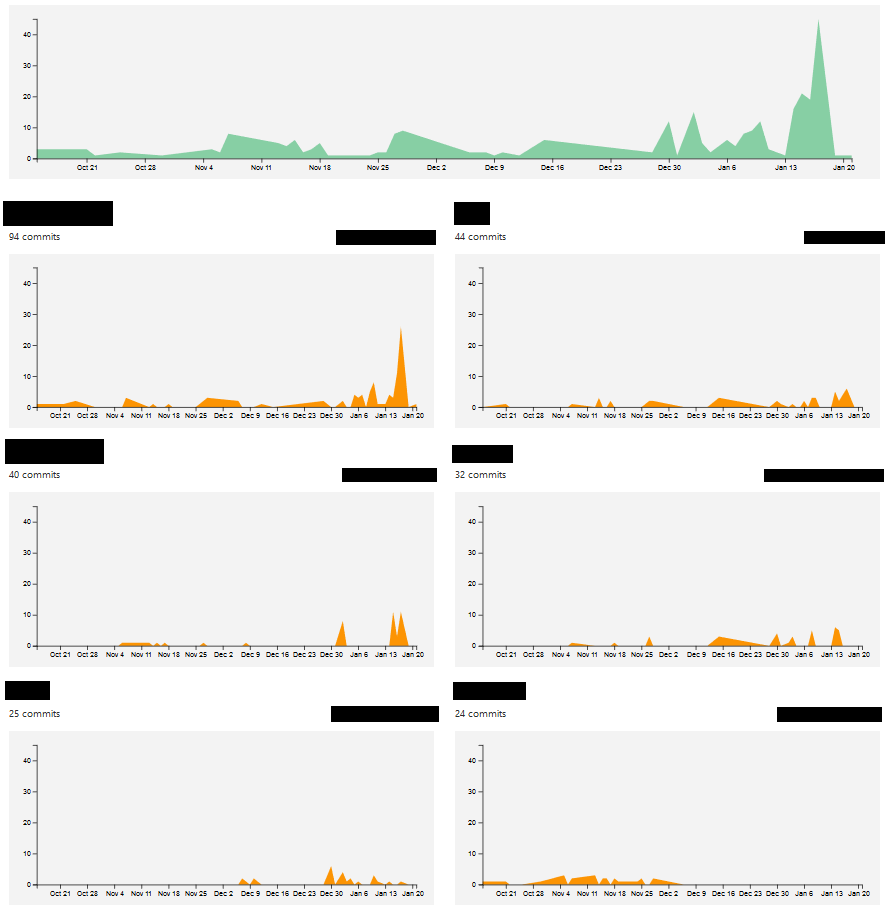
\includegraphics[scale=0.4]{slike/aktivnost.PNG} %veličina slike u odnosu na originalnu datoteku i pozicija slike
%			\centering
%			\caption{Primjer slike s potpisom}
%			\label{fig:promjene}
%		\end{figure}
%		
%		\begin{figure}[H]
%			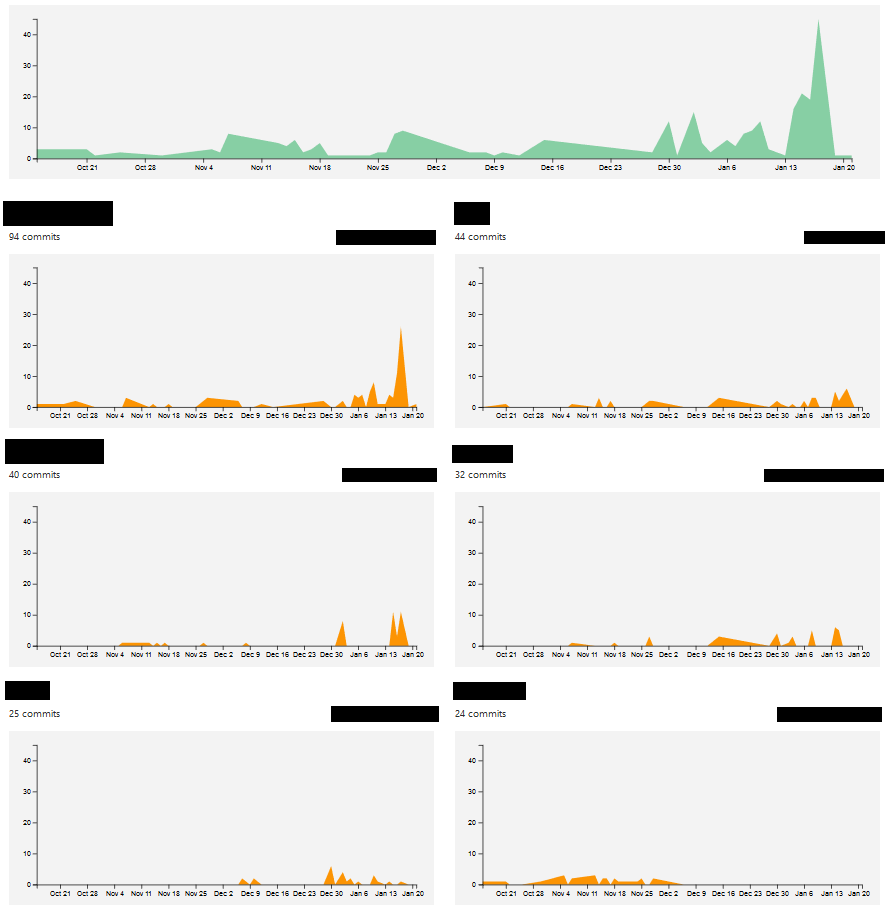
\includegraphics[width=\textwidth]{slike/aktivnost.PNG} %veličina u odnosu na širinu linije
%			\caption{Primjer slike s potpisom 2}
%			\label{fig:promjene2} %label mora biti drugaciji za svaku sliku
%		\end{figure}
%		
%		Referenciranje slike \ref{fig:promjene2} u tekstu.
%		
%		\eject
%		
	
	\chapter{Specifikacija programske potpore}
		
	\section{Funkcionalni zahtjevi}
			
			%\textbf{\textit{dio 1. revizije}}\\
			
			%\textit{Navesti \textbf{dionike} koji imaju \textbf{interes u ovom sustavu} ili  \textbf{su nositelji odgovornosti}. To su prije svega korisnici, ali i administratori sustava, naručitelji, razvojni tim.}\\
				
			%\textit{Navesti \textbf{aktore} koji izravno \textbf{koriste} ili \textbf{komuniciraju sa sustavom}. Oni mogu imati inicijatorsku ulogu, tj. započinju određene procese u sustavu ili samo sudioničku ulogu, tj. obavljaju određeni posao. Za svakog aktora navesti funkcionalne zahtjeve koji se na njega odnose.}\\
			
			
			\noindent \textbf{Dionici:}
			
			\begin{packed_enum}
				
				\item Korisnici
				\item[]\begin{packed_enum}
					\item Neregistrirani korisnici
					\item Klijenti
					\item Kulinarski entuzijasti
					\item Nutricionisti
				\end{packed_enum}
				\item Administratori
				\item Razvojni tim
				
			\end{packed_enum}
			
			\noindent \textbf{Aktori i njihovi funkcionalni zahtjevi:}
			
			\begin{packed_enum}
				\item  \underbar{Neregistrirani korisnik (inicijator) može:}
				
				\begin{packed_enum}
					
					\item Pregledavati kuharice sortirane po novosti na prednjoj stranici
					\item Poslati zahtjev za registraciju:
					\begin{packed_enum}
						
						\item  Za klijenta s korisničkim imenom, lozinkom te imenom i prezimenom 
						\item  Za kulinarskog entuzijasta ili nutricionista sa dodatnom slikom, e-adresom i kratkom biografijom
				
					\end{packed_enum}
					\item  Pretraživati profile kulinarskih entuzijasta
					\item Pretraživati i anonimno komentirati kuharice
					
				\end{packed_enum}

				\item  \underbar{Klijent (inicijator) može:}
				
				\begin{packed_enum}
					
					\item Sve što i neregistrirani korisnik, osim slanja zahtjeva zahtjeva za registraciju
					\item Odabrati dijetu koju prate
					\item Pretraživati recepte skeniranjem QR koda proizvoda
					\item Označiti konzumirane recepte
					\item Komentirati kuharice
					
				\end{packed_enum}
				
				\item  \underbar{Kulinarski entuzijast (inicijator) može:}
				
				\begin{packed_enum}
					
					\item Sve što i klijent
					\item Kreirati recepte i kuharice, to jest tematski povezane skupove recepata
					
				\end{packed_enum}

				\item  \underbar{Nutricionist (inicijator) može:}
				
				\begin{packed_enum}
					
					\item Sve što i klijent
					\item Unositi informacije o proizvodima
					\item Kategorizirati proizvode
					\item Kreirati dijete
					
				\end{packed_enum}

				\item  \underbar{Administrator (inicijator) može:}
				
				\begin{packed_enum}
					
					\item Sve što i klijent, nutricionist i kulinarski entuzijast
					\item Odobriti prijave nutricionista i kulinarskih entuzijasta
					\item Pisati u i čitati iz baze podataka
					
				\end{packed_enum}

				\item  \underbar{Baza podataka (sudionik) može:}
	
				\begin{packed_enum}
					
					\item Brinuti se da je zadovoljen model podataka
					\item čuvati trenutno stanje korisnika, kuharica, dijeti i recepata
					
				\end{packed_enum}
			\end{packed_enum}
			
			\eject 

%			\begin{packed_enum}
%				\item  \underbar{Aktor 1 (inicijator) može:}
%				
%				\begin{packed_enum}
%					
%					\item funkcionalnost 1
%					\item funkcionalnost 2
%					\begin{packed_enum}
%						
%						\item  podfunkcionalnost 1 
%						\item  podfunkcionalnost 2
%				
%					\end{packed_enum}
%					\item  funkcionalnost 3
%					
%				\end{packed_enum}
%			
%				\item  \underbar{Aktor 2 (sudionik) može:}
%				
%				\begin{packed_enum}
%					
%					\item funkcionalnost 1
%					\item funkcionalnost 2
%					
%				\end{packed_enum}
%			\end{packed_enum}
%			
%			\eject 

				
			\subsection{Obrasci uporabe}
%				
%				\textbf{\textit{dio 1. revizije}}
%				
				\subsubsection{Opis obrazaca uporabe}
					\noindent \underbar{\textbf{UC1 - Pregled novih kuharica}}
					\begin{packed_item}
	
						\item \textbf{Glavni sudionik: }Neregistrirani korisnik, Klijent, Kulinarski entuzijast, Administrator
						\item  \textbf{Cilj:} Pregledavanje kuharica
						\item  \textbf{Sudionici:} Baza podataka
						\item  \textbf{Preduvjet:} -
						\item  \textbf{Opis osnovnog tijeka:} 
						
						\item[] \begin{packed_enum}
	
							\item Nove kuharice su prikazane prilikom učitavanja aplikacije
							\item Korisnik odabire jednu od navedenih kuharica
							\item Prikazuje se lista recepata unutar navedene kuharice
						\end{packed_enum}
						
						\item  \textbf{Opis mogućih odstupanja:}
						
						\item[] \begin{packed_item}
	
							\item[2.a] Nema kuharica u bazi podataka
							\item[] \begin{packed_enum}
								
								\item Sustav ispisuje poruku da nema kuharica u bazi podataka
								
							\end{packed_enum}

							
						\end{packed_item}
					\end{packed_item}



					\noindent \underbar{\textbf{UC2 - Registracija klijenta}}
					\begin{packed_item}
	
						\item \textbf{Glavni sudionik: }Neregistrirani korisnik
						\item  \textbf{Cilj:} Stvaranje korisničkog računa s statusom klijenta
						\item  \textbf{Sudionici:} Baza podataka
						\item  \textbf{Preduvjet:} -
						\item  \textbf{Opis osnovnog tijeka:} 
						
						\item[] \begin{packed_enum}
	
							\item pritiskom na gumb "Sign up" otvara se sučelje za registraciju
							\item Korisnik unosi podatke o korisničkom imenu, lozinki, imenu i prezimenu
							\item Korisnik prima obavijest o uspješnoj registraciji
						\end{packed_enum}
						
						\item  \textbf{Opis mogućih odstupanja:}
						
						\item[] \begin{packed_item}
	
							\item[2.a] Odabir već zauzetog korisničkog imena, unos korisničkog podatka u nedozvoljenom formatu
							\item[] \begin{packed_enum}
								
								\item Sustav obavještava korisnika o neuspjeloj registraciji i vraća ga u sučelje za registraciju
								\item Korisnik mijenja potrebne podatke i završava registraciju ili odustaje od registracije
								
							\end{packed_enum}

							
						\end{packed_item}
					\end{packed_item}



					\noindent \underbar{\textbf{UC3 - Registracija kulinarskog entuzijasta ili nutricionista}}
					\begin{packed_item}
	
						\item \textbf{Glavni sudionik: }Neregistrirani korisnik
						\item  \textbf{Cilj:} Stvaranje korisničkog računa s statusom kulinarskog entuzijasta ili nutricionista
						\item  \textbf{Sudionici:} Baza podataka, Administrator
						\item  \textbf{Preduvjet:} -
						\item  \textbf{Opis osnovnog tijeka:} 
						
						\item[] \begin{packed_enum}
	
							\item pritiskom na gumb "Sign up" otvara se sučelje za registraciju
							\item Korisnik unosi podatke o korisničkom imenu, lozinki, imenu i prezimenu, e-adresom, kratkom biografijom i slikom
							\item Korisnik prima obavijest o uspješnoj registraciji nakon odobrenja administratora
						\end{packed_enum}
						
						\item  \textbf{Opis mogućih odstupanja:}
						
						\item[] \begin{packed_item}
	
							\item[2.a] Odabir već zauzetog korisničkog imena i/ili e-maila, unos korisničkog podatka u nedozvoljenom formatu
							\item[] \begin{packed_enum}
								
								\item Sustav obavještava korisnika o neuspjeloj registraciji i vraća ga u sučelje za registraciju
								\item Korisnik mijenja potrebne podatke i završava registraciju ili odustaje od registracije
								
							\end{packed_enum}
							\item[2.b] Administrator ne odobrava registraciju
							\item[] \begin{packed_enum}
								
								\item Sustav obavještava korisnika o neuspjeloj registraciji i vraća ga u sučelje za registraciju
								\item Korisnik mijenja potrebne podatke i završava registraciju ili odustaje od registracije
								
							\end{packed_enum}
							
						\end{packed_item}
					\end{packed_item}



					\noindent \underbar{\textbf{UC4 - Pregled profila kulinarskih entuzijasta}}
					\begin{packed_item}
	
						\item \textbf{Glavni sudionik: }Neregistrirani korisnik, Klijent, Kulinarski entuzijast, Nutricionist, Administrator
						\item  \textbf{Cilj:} Pregled profila kulinarskih entuzijasta
						\item  \textbf{Sudionici:} Baza podataka
						\item  \textbf{Preduvjet:} -
						\item  \textbf{Opis osnovnog tijeka:} 
						
						\item[] \begin{packed_enum}
	
							\item korisnik odabire ime kulinarskog entuzijasta unutar kuharice
							\item Otvara se sučelje s podatcima o kulinarskom entuzijastu
						\end{packed_enum}
						

					\end{packed_item}



					\noindent \underbar{\textbf{UC5 - Pretraživanje profila kulinarskih entuzijasta i kuharica}}
					\begin{packed_item}
	
						\item \textbf{Glavni sudionik: }Neregistrirani korisnik, Klijent, Kulinarski entuzijast, Nutricionist, Administrator
						\item  \textbf{Cilj:} Pregled profila i kuharica koje sadrže ključnu riječ
						\item  \textbf{Sudionici:} Baza podataka
						\item  \textbf{Preduvjet:} -
						\item  \textbf{Opis osnovnog tijeka:} 
						
						\item[] \begin{packed_enum}
	
							\item korisnik u tražilicu upisuje jednu ili više ključnih riječi 
							\item Korisnik odabire gumb za pretraživanje
							\item Otvara se sučelje s listom profila i kuharica koje sadrže ključne riječi
						\end{packed_enum}
						
						\item  \textbf{Opis mogućih odstupanja:}
						
						\item[] \begin{packed_item}
	
							\item[2.a] Niti jedan profil ili kuharica ne sadrži ključnu riječ
							\item[] \begin{packed_enum}
								
								\item Sustav obavještava korisnika o neuspjelom pretraživanju 
								\item Klijent se vrati u sučelje gdje je bio prije pretraživanja
								
							\end{packed_enum}

							\item[2.b] Nije upisana ključna riječ prije pretraživanja
							\item[] \begin{packed_enum}
								
								\item Sustav obavještava korisnika o neuspjelom pretraživanju 
								\item Klijent se vrati u sučelje gdje je bio prije pretraživanja
								
							\end{packed_enum}							
						\end{packed_item}
					\end{packed_item}



					\noindent \underbar{\textbf{UC6 - Anonimno komentiranje kuharica}}
					\begin{packed_item}
	
						\item \textbf{Glavni sudionik: }Neregistrirani korisnik
						\item  \textbf{Cilj:} Komentiranje kuharica
						\item  \textbf{Sudionici:} Baza podataka
						\item  \textbf{Preduvjet:} -
						\item  \textbf{Opis osnovnog tijeka:} 
						
						\item[] \begin{packed_enum}
	
							\item korisnik unutar kuharice odabire gumb "Komentiraj"
							\item Otvara se sučelje gdje korisnik upisuje tekst
							\item Pritiskom na gumb "Spremi", komentar se sprema u bazu podataka i vidljiv je unutar kuharice
						\end{packed_enum}
						
						\item  \textbf{Opis mogućih odstupanja:}
						
						\item[] \begin{packed_item}
	
							\item[2.a] Pokušaj spremanja praznog komentara
							\item[] \begin{packed_enum}
								
								\item Sustav obavještava korisnika o neuspjelom pokušaju spremanja komentara 
								\item Klijent ispuni polje za komentar ili odustane
								
							\end{packed_enum}

						\end{packed_item}
					\end{packed_item}



					\noindent \underbar{\textbf{UC7 - Prijava u sustav}}
					\begin{packed_item}
	
						\item \textbf{Glavni sudionik: } Klijent, Kulinarski entuzijast, Nutricionist, Administrator
						\item  \textbf{Cilj:} Prijava u sustav kao registrirani korisnik
						\item  \textbf{Sudionici:} Baza podataka
						\item  \textbf{Preduvjet:} Registracija profila
						\item  \textbf{Opis osnovnog tijeka:} 
						
						\item[] \begin{packed_enum}
	
							\item Korisnik odabire opciju "Prijavi se"
							\item Korisnik ispunjava potrebne podatke
							\item Korisnik je prijavljen i vraća se na početnu stranicu
						\end{packed_enum}
						
						\item  \textbf{Opis mogućih odstupanja:}
						
						\item[] \begin{packed_item}
	
							\item[2.a] Neispravni unos podataka
							\item[] \begin{packed_enum}
								
								\item Sustav obavještava korisnika o neispravnim podatcima i traži ponovni unos podataka
								
							\end{packed_enum}

						\end{packed_item}
					\end{packed_item}


					\noindent \underbar{\textbf{UC8 - Odabir dijete koje će korisnik pratiti}}
					\begin{packed_item}
	
						\item \textbf{Glavni sudionik: }Klijent, Kulinarski entuzijast, Nutricionist, Administrator 
						\item  \textbf{Cilj:} Odabir dijete
						\item  \textbf{Sudionici:} Baza podataka
						\item  \textbf{Preduvjet:} -
						\item  \textbf{Opis osnovnog tijeka:} 
						
						\item[] \begin{packed_enum}
	
							\item korisnik odabire gumb "Odabir dijete"
							\item Otvara se sučelje gdje korisnik odabire jednu od navedenih dijeta
							\item Pritiskom na gumb "Spremi", odabrana dijeta se sprema i vidljiva je u receptima koje korisnik pregledava ili filtrira recepte koji zadovoljavaju dijetu
						\end{packed_enum}
						
						\item  \textbf{Opis mogućih odstupanja:}
						
						\item[] \begin{packed_item}
	
							\item[2.a] Pokušaj spremanja bez odabira dijete
							\item[] \begin{packed_enum}
								
								\item Sustav obavještava korisnika o neuspjelom pokušaju spremanja dijete
								\item Klijent ispuni polje za dijetu ili odustane
								
							\end{packed_enum}							
							\item[2.b] Nema dijeta u sustavu
							\item[] \begin{packed_enum}
								
								\item Sustav obavještava korisnika o nedostatku dijeta
								
							\end{packed_enum}

						\end{packed_item}
					\end{packed_item}





					\noindent \underbar{\textbf{UC9 - Pretraživanje unosom QR koda}}
					\begin{packed_item}
	
						\item \textbf{Glavni sudionik: }Klijent, Kulinarski entuzijast, Nutricionist, Administrator 
						\item  \textbf{Cilj:} Na temelju koda na proizvodu vidjeti recepte u kojima se on nalazi
						\item  \textbf{Sudionici:} Baza podataka
						\item  \textbf{Preduvjet:} -
						\item  \textbf{Opis osnovnog tijeka:} 
						
						\item[] \begin{packed_enum}
	
						\item Korisnik bira opciju "Skeniraj kod proizvoda"
						\item Korisnik je poslan na stranicu s opcijom postavljanja slike na poslužitelj
						\item Korisnik postavlja sliku i čeka njenu obradu
						\item Korisnik dobiva popis recepata koji sadrže skenirani proizvod
						\end{packed_enum}
						
						\item  \textbf{Opis mogućih odstupanja:}
						
						\item[] \begin{packed_item}
	
							\item[2.a] Slika nije u podržanom formatu
							\item[] \begin{packed_enum}
								
								\item Sustav ispisuje poruku da slika nije u podržanom formatu i traži se ponovni unos slike
								
							\end{packed_enum}							
							\item[2.b] Kod u slici nije pronađen
							\item[] \begin{packed_enum}
								
								\item Sustav ispisuje poruku da kod na slici nije prepoznat i traži se ponovni unos slike
								
							\end{packed_enum}

						\end{packed_item}
					\end{packed_item}



					\noindent \underbar{\textbf{UC10 - Kreiranje kuharice}}
					\begin{packed_item}
	
						\item \textbf{Glavni sudionik: } Kulinarski entuzijast, Administrator 
						\item  \textbf{Cilj:} Kreirati kuharicu koja sadrži različite recepte
						\item  \textbf{Sudionici:} Baza podataka
						\item  \textbf{Preduvjet:} -
						\item  \textbf{Opis osnovnog tijeka:} 
						
						\item[] \begin{packed_enum}
	
						\item Korisnik bira opciju "Kreiraj kuharicu" nakon čega se otvara sučelje za kreiranje kuharice
						\item Korisnik odabire gumb "Dodaj recept" i odabire recept koji će dodati u kuharicu				
						\item Korisnik odabire gumb "Obriši recept" i odabire recept koji će se maknuti iz kuharice
						\item Korisnik odabire gumb "Spremi kuharicu" čime se kuharica sprema u bazu podataka
						\end{packed_enum}
						
						\item  \textbf{Opis mogućih odstupanja:}
						
						\item[] \begin{packed_item}
	
							\item[2.a] Spremanje prazne kuharice
							\item[] \begin{packed_enum}
								
								\item Sustav ispisuje poruku da nema recepata u kuharici
								\item Korisnik dodaje recepte kuharicu ili odustaje
								
							\end{packed_enum}							


						\end{packed_item}
					\end{packed_item}


					\noindent \underbar{\textbf{UC11 - Uređivanje kuharice}}
					\begin{packed_item}
	
						\item \textbf{Glavni sudionik: } Kulinarski entuzijast, Administrator 
						\item  \textbf{Cilj:} Uređivanje jedne od vlastitih kuharica
						\item  \textbf{Sudionici:} Baza podataka
						\item  \textbf{Preduvjet:} -
						\item  \textbf{Opis osnovnog tijeka:} 
						
						\item[] \begin{packed_enum}
	
						\item Korisnik bira opciju "Uredi kuharicu" nakon čega se otvara sučelje za uređivanje kuharice
						\item Korisnik odabire gumb "Dodaj recept" i odabire recept koji će dodati u kuharicu				
						\item Korisnik odabire gumb "Obriši recept" i odabire recept koji će se maknuti iz kuharice
						\item Korisnik odabire gumb "Spremi kuharicu" čime se kuharica sprema u bazu podataka
						\end{packed_enum}
						
						\item  \textbf{Opis mogućih odstupanja:}
						
						\item[] \begin{packed_item}
	
							\item[2.a] Spremanje prazne kuharice
							\item[] \begin{packed_enum}
								
								\item Sustav ispisuje poruku da nema recepata u kuharici
								\item Korisnik dodaje recepte kuharicu ili odustaje
								
							\end{packed_enum}							


						\end{packed_item}
					\end{packed_item}



					\noindent \underbar{\textbf{UC12 - Kreiranje recepata}}
					\begin{packed_item}
	
						\item \textbf{Glavni sudionik: } Kulinarski entuzijast, Administrator 
						\item  \textbf{Cilj:} Kreirati kuharicu koja sadrži različite recepte
						\item  \textbf{Sudionici:} Baza podataka
						\item  \textbf{Preduvjet:} -
						\item  \textbf{Opis osnovnog tijeka:} 
						
						\item[] \begin{packed_enum}
	
						\item Korisnik bira opciju "Kreiraj recept" nakon čega se otvara sučelje za kreiranje recepata
						\item Korisnik odabire sastojke koji ulaze u recept i upisuje način pripreme jela
						\item Korisnik odabire gumb "Spremi recept" čime se recept sprema u bazu podataka
						\end{packed_enum}
						
						\item  \textbf{Opis mogućih odstupanja:}
						
						\item[] \begin{packed_item}
	
							\item[2.a] Spremanje praznog recepta
							\item[] \begin{packed_enum}
								
								\item Sustav ispisuje poruku da nema sastojaka ili opisa pripreme
								\item Korisnik dodaje potrebne informacije ili odustaje
								
							\end{packed_enum}							


						\end{packed_item}
					\end{packed_item}


					\noindent \underbar{\textbf{UC13 - Uređivanje recepata}}
					\begin{packed_item}
	
						\item \textbf{Glavni sudionik: } Kulinarski entuzijast, Administrator 
						\item  \textbf{Cilj:} Uređivanje jednog od vlastitih recepata
						\item  \textbf{Sudionici:} Baza podataka
						\item  \textbf{Preduvjet:} -
						\item  \textbf{Opis osnovnog tijeka:} 
						
						\item[] \begin{packed_enum}
	
						\item Korisnik bira opciju "Uredi recept" nakon čega se otvara sučelje za uređivanje recepata
						\item Korisnik mijenja sastojke koji ulaze u recept i mijenja opis pripreme
						\item Korisnik odabire gumb "Spremi recept" čime se recept sprema u bazu podataka
						\end{packed_enum}
						
						\item  \textbf{Opis mogućih odstupanja:}
						
						\item[] \begin{packed_item}
	
							\item[2.a] Spremanje praznog recepta
							\item[] \begin{packed_enum}
								
								\item Sustav ispisuje poruku da nema sastojaka ili opisa pripreme
								\item Korisnik dodaje potrebne informacije ili odustaje
								
							\end{packed_enum}						


						\end{packed_item}
					\end{packed_item}

                    \noindent \underbar{\textbf{UC14 - Unošenje proizvoda}}
                    \begin{packed_item}
    
                        \item \textbf{Glavni sudionik: }Nutricionist, Administrator
                        \item  \textbf{Cilj:} Unošenje novog proizvoda zajedno sa relevantnim atributima
                        \item  \textbf{Sudionici:} Baza podataka
                        \item  \textbf{Preduvjet:} Nema navedenog proizvoda u bazi podataka
                        \item  \textbf{Opis osnovnog tijeka:} 
                        
                        \item[] \begin{packed_enum}
    
                            \item Korisnik pritisne gumb "Dodaj proizvod"
                            \item Prikazuje se sučelje u koje korisnik upisuje potrebne podatke
                            \item Korisnik pritisne gumb "Spremi" kojim sprema proizvod zajedno sa vezanim informacijama u bazu podataka
                        \end{packed_enum}
                        
                        \item  \textbf{Opis mogućih odstupanja:}
                        
                        \item[] \begin{packed_item}
    
                            \item[2.a] Proizvod tog imena već postoji u bazi podataka
                            \item[] \begin{packed_enum}
                                
                                \item Sustav ispisuje poruku da je proizvod istog imena već u bazi podataka
                                \item Korisnik mijenja naziv proizvoda ili odustane
                                
                            \end{packed_enum}

                            \item[2.b] Unos informacija u nedozvoljenom formatu
                            \item[] \begin{packed_enum}
                                
                                \item Sustav ispisuje poruku s dojavom greške
                                \item Korisnik mijenja informacije ili odustane
                                
                            \end{packed_enum}

                        \end{packed_item}
                    \end{packed_item}

                    \noindent \underbar{\textbf{UC15 - Promjena informacija o proizvodima}}
                    \begin{packed_item}
    
                        \item \textbf{Glavni sudionik: }Nutricionist, Administrator
                        \item  \textbf{Cilj:} Promjena atributa postojećeg proizvoda
                        \item  \textbf{Sudionici:} Baza podataka
                        \item  \textbf{Preduvjet:} Postoji navedeni proizvod u bazi podataka
                        \item  \textbf{Opis osnovnog tijeka:} 
                        
                        \item[] \begin{packed_enum}
    
                            \item Korisnik pritisne gumb "Promijeni proizvod"
                            \item Prikazuje se sučelje u koje korisnik mijenja podatke proizvoda
                            \item Korisnik pritisne gumb "Spremi" kojim sprema proizvod zajedno sa promjenjenim informacijama u bazu podataka
                        \end{packed_enum}
                        
                        \item  \textbf{Opis mogućih odstupanja:}
                        
                        \item[] \begin{packed_item}
    
                            \item[2.a] Unos informacija u nedozvoljenom formatu
                            \item[] \begin{packed_enum}
                                
                                \item Sustav ispisuje poruku s dojavom greške
                                \item Korisnik mijenja informacije ili odustane
                                
                            \end{packed_enum}

                            
                        \end{packed_item}
                    \end{packed_item}

                    \noindent \underbar{\textbf{UC16 - Brisanje proizvoda}}
                    \begin{packed_item}
    
                        \item \textbf{Glavni sudionik: }Nutricionist, Administrator
                        \item  \textbf{Cilj:} Brisanje postojećeg proizvoda
                        \item  \textbf{Sudionici:} Baza podataka
                        \item  \textbf{Preduvjet:} Postoji navedeni proizvod u bazi podataka
                        \item  \textbf{Opis osnovnog tijeka:} 
                        
                        \item[] \begin{packed_enum}
    
                            \item Korisnik pritisne gumb "Briši proizvod"
                            \item Prikazuje se sučelje u kojemu se daje korisniku opcija "Briši" ili "Odustani"
                            \item Korisnik pritisne gumb "Briši" čime se briše proizvod iz baze podataka ili pritisne gumb "Odustani" čime se zaustavi brisanje proizvoda
                        \end{packed_enum}
                        
                    \end{packed_item}

                    \noindent \underbar{\textbf{UC17 - Kategorizirati proizvode}}
                    \begin{packed_item}
    
                        \item \textbf{Glavni sudionik: }Nutricionist, Administrator
                        \item  \textbf{Cilj:} Dodavanje kategorije postojećem proizvodu
                        \item  \textbf{Sudionici:} Baza podataka
                        \item  \textbf{Preduvjet:} Postoji navedeni proizvod u bazi podataka
                        \item  \textbf{Opis osnovnog tijeka:} 
                        
                        \item[] \begin{packed_enum}
    
                            \item Korisnik pritisne gumb "Kategoriziraj proizvod"
                            \item Prikazuje se sučelje u koje korisnik dodaje ili mijenja kategoriju proizvoda
                            \item Korisnik pritisne gumb "Spremi" kojim sprema kategoriju proizvoda u bazu podataka
                        \end{packed_enum}
                        
                        \item  \textbf{Opis mogućih odstupanja:}
                        
                        \item[] \begin{packed_item}
    
                            \item[2.a] Unos informacija u nedozvoljenom formatu
                            \item[] \begin{packed_enum}
                                
                                \item Sustav ispisuje poruku s dojavom greške
                                \item Korisnik mijenja informacije ili odustane
                                
                            \end{packed_enum}

                            
                        \end{packed_item}
                    \end{packed_item}

                    \noindent \underbar{\textbf{UC18 - Dodavanje kategorija}}
                    \begin{packed_item}
    
                        \item \textbf{Glavni sudionik: }Nutricionist, Administrator
                        \item  \textbf{Cilj:} Dodavanje nove kategorije
                        \item  \textbf{Sudionici:} Baza podataka
                        \item  \textbf{Preduvjet:} Nema navedene kategorije u bazi podataka
                        \item  \textbf{Opis osnovnog tijeka:} 
                        
                        \item[] \begin{packed_enum}
    
                            \item Korisnik pritisne gumb "Dodaj kategoriju"
                            \item Prikazuje se sučelje u koje korisnik dodaje kategoriju
                            \item Korisnik pritisne gumb "Spremi" kojim sprema kategoriju proizvoda u bazu podataka
                        \end{packed_enum}
                        
                        \item  \textbf{Opis mogućih odstupanja:}
                        
                        \item[] \begin{packed_item}
    
                            \item[2.a] Kategorija tog imena već postoji u bazi podataka
                            \item[] \begin{packed_enum}
                                
                                \item Sustav ispisuje poruku da je kategorija istog imena već u bazi podataka
                                \item Korisnik mijenja naziv kategorije ili odustane
                                
                            \end{packed_enum}

                            \item[2.b] Unos informacija u nedozvoljenom formatu
                            \item[] \begin{packed_enum}
                                
                                \item Sustav ispisuje poruku s dojavom greške
                                \item Korisnik mijenja informacije ili odustane
                                
                            \end{packed_enum}

                            
                        \end{packed_item}
                    \end{packed_item}

                    \noindent \underbar{\textbf{UC19 - Promjena kategorije}}
                    \begin{packed_item}
    
                        \item \textbf{Glavni sudionik: }Nutricionist, Administrator
                        \item  \textbf{Cilj:} Promjena atributa kategorije
                        \item  \textbf{Sudionici:} Baza podataka
                        \item  \textbf{Preduvjet:} Postoji navedena kategorija u bazi podataka
                        \item  \textbf{Opis osnovnog tijeka:} 
                        
                        \item[] \begin{packed_enum}
    
                            \item Korisnik pritisne gumb "Promijeni kategoriju"
                            \item Prikazuje se sučelje gdje korisnik mijenja atribute kategorije
                            \item Korisnik pritisne gumb "Spremi" kojim sprema promjene u bazu podataka
                        \end{packed_enum}
                        
                        \item  \textbf{Opis mogućih odstupanja:}
                        
                        \item[] \begin{packed_item}

                            \item[2.a] Unos informacija u nedozvoljenom formatu
                            \item[] \begin{packed_enum}
                                
                                \item Sustav ispisuje poruku s dojavom greške
                                \item Korisnik mijenja informacije ili odustane
                                
                            \end{packed_enum}

                            
                        \end{packed_item}
                    \end{packed_item}

                    \noindent \underbar{\textbf{UC20 - Brisanje kategorija}}
                    \begin{packed_item}
    
                        \item \textbf{Glavni sudionik: }Nutricionist, Administrator
                        \item  \textbf{Cilj:} Brisanje postojeće kategorije
                        \item  \textbf{Sudionici:} Baza podataka
                        \item  \textbf{Preduvjet:} Postoji navedena kategorije u bazi podataka
                        \item  \textbf{Opis osnovnog tijeka:} 
                        
                        \item[] \begin{packed_enum}
    
                            \item Korisnik pritisne gumb "Briši kategoriju"
                            \item Prikazuje se sučelje u kojemu se daje korisniku opcija "Briši" ili "Odustani"
                            \item Korisnik pritisne gumb "Briši" čime se briše kategorija iz baze podataka ili pritisne gumb "Odustani" čime se zaustavi brisanje kategorije
                        \end{packed_enum}
                        
                    \end{packed_item}


                    \noindent \underbar{\textbf{UC21 - Dodavanje dijeta}}
                    \begin{packed_item}
    
                        \item \textbf{Glavni sudionik: }Nutricionist, Administrator
                        \item  \textbf{Cilj:} Dodavanje nove dijete
                        \item  \textbf{Sudionici:} Baza podataka
                        \item  \textbf{Preduvjet:} Nema navedene dijete u bazi podataka
                        \item  \textbf{Opis osnovnog tijeka:} 
                        
                        \item[] \begin{packed_enum}
    
                            \item Korisnik pritisne gumb "Dodaj dijetu"
                            \item Prikazuje se sučelje u koje korisnik dodaje dijetu
                            \item Korisnik pritisne gumb "Spremi" kojim sprema dijetu u bazu podataka
                        \end{packed_enum}
                        
                        \item  \textbf{Opis mogućih odstupanja:}
                        
                        \item[] \begin{packed_item}
    
                            \item[2.a] Dijeta tog imena već postoji u bazi podataka
                            \item[] \begin{packed_enum}
                                
                                \item Sustav ispisuje poruku da je dijeta istog imena već u bazi podataka
                                \item Korisnik mijenja naziv dijete ili odustane
                                
                            \end{packed_enum}

                            \item[2.b] Unos informacija u nedozvoljenom formatu
                            \item[] \begin{packed_enum}
                                
                                \item Sustav ispisuje poruku s dojavom greške
                                \item Korisnik mijenja informacije ili odustane
                                
                            \end{packed_enum}

                            
                        \end{packed_item}
                    \end{packed_item}

                    \noindent \underbar{\textbf{UC22 - Promjena dijeta}}
                    \begin{packed_item}
    
                        \item \textbf{Glavni sudionik: }Nutricionist, Administrator
                        \item  \textbf{Cilj:} Promjena atributa i stavki dijete
                        \item  \textbf{Sudionici:} Baza podataka
                        \item  \textbf{Preduvjet:} Postoji navedena kategorija u bazi podataka
                        \item  \textbf{Opis osnovnog tijeka:} 
                        
                        \item[] \begin{packed_enum}
    
                            \item Korisnik pritisne gumb "Promijeni dijetu"
                            \item Prikazuje se sučelje gdje korisnik mijenja atribute i stavke dijete
                            \item Korisnik pritisne gumb "Spremi" kojim sprema promjene u bazu podataka
                        \end{packed_enum}
                        
                        \item  \textbf{Opis mogućih odstupanja:}
                        
                        \item[] \begin{packed_item}

                            \item[2.a] Unos informacija u nedozvoljenom formatu
                            \item[] \begin{packed_enum}
                                
                                \item Sustav ispisuje poruku s dojavom greške
                                \item Korisnik mijenja informacije ili odustane
                                
                            \end{packed_enum}

                            
                        \end{packed_item}
                    \end{packed_item}

                    \noindent \underbar{\textbf{UC23 - Brisanje dijeta}}
                    \begin{packed_item}
    
                        \item \textbf{Glavni sudionik: }Nutricionist, Administrator
                        \item  \textbf{Cilj:} Brisanje postojeće dijete
                        \item  \textbf{Sudionici:} Baza podataka
                        \item  \textbf{Preduvjet:} Postoji navedena dijeta u bazi podataka
                        \item  \textbf{Opis osnovnog tijeka:} 
                        
                        \item[] \begin{packed_enum}
    
                            \item Korisnik pritisne gumb "Briši dijetu"
                            \item Prikazuje se sučelje u kojemu se daje korisniku opcija "Briši" ili "Odustani"
                            \item Korisnik pritisne gumb "Briši" čime se briše dijeta iz baze podataka ili pritisne gumb "Odustani" čime se zaustavi brisanje dijete
                        \end{packed_enum}
                        
                    \end{packed_item}

                    \noindent \underbar{\textbf{UC24 - Prihvaćanje ili odbijanje prijave nutricionista i kulinarskih entuzijasta}}
                    \begin{packed_item}
    
                        \item \textbf{Glavni sudionik: }Administrator
                        \item  \textbf{Cilj:} Odobriti ili poništiti zahtjev za ulogu nutricionista ili kulinarskog entuzijasta korisniku
                        \item  \textbf{Sudionici:} Baza podataka
                        \item  \textbf{Preduvjet:} Postoji prijava za ulogu nutricionista ili kulinarskog entuzijasta
                        \item  \textbf{Opis osnovnog tijeka:} 
                        
                        \item[] \begin{packed_enum}
    
                            \item Korisnik pritisne gumb "Provjeri prijavu"
                            \item Prikazuje se sučelje u kojemu se daje korisniku opcija "Prihvati" ili "Odbij"
                            \item Korisnik pritisne gumb "Prihvati" čime se prihvaća prijava korisnika za ulogu u bazi podataka ili pritisne gumb "Odbij" čime se odbija prijava korisnika za traženu ulogu
                        \end{packed_enum}
                        
                    \end{packed_item}  					



			\noindent \underbar{\textbf{UC25 - Komentiranje kuharica}}
					\begin{packed_item}
	
						\item \textbf{Glavni sudionik: }Klijent, Kulinarski entuzijast, Nutricionist, Administrator 
						\item  \textbf{Cilj:} Komentiranje kuharica
						\item  \textbf{Sudionici:} Baza podataka
						\item  \textbf{Preduvjet:} -
						\item  \textbf{Opis osnovnog tijeka:} 
						
						\item[] \begin{packed_enum}
	
							\item korisnik unutar kuharice odabire gumb "Komentiraj"
							\item Otvara se sučelje gdje korisnik upisuje tekst
							\item Pritiskom na gumb "Spremi", komentar se sprema u bazu podataka i vidljiv je unutar kuharice
						\end{packed_enum}
						
						\item  \textbf{Opis mogućih odstupanja:}
						
						\item[] \begin{packed_item}
	
							\item[2.a] Pokušaj spremanja praznog komentara
							\item[] \begin{packed_enum}
								
								\item Sustav obavještava korisnika o neuspjelom pokušaju spremanja komentara 
								\item Klijent ispuni polje za komentar ili odustane
								
							\end{packed_enum}

						\end{packed_item}
					\end{packed_item}




%%
%                   \noindent \underbar{\textbf{UC9 - Pretraživanje unosom QR koda}}
%                    \begin{packed_item}
%
%                        \item \textbf{Glavni sudionik: }Klijent
%                        \item  \textbf{Cilj:}Na temelju koda na proizvodu vidjeti recepte u kojima se on nalazi
%                        \item  \textbf{Sudionici:} Baza podataka
%                        \item  \textbf{Preduvjet:} Klijent je prijavljen
%                        \item  \textbf{Opis osnovnog tijeka:}
%
%                        \item[] \begin{packed_enum}
%
% 						\item Korisnik bira opciju "Skeniraj kod proizvoda"
%						\item Korisnik je poslan na stranicu s opcijom postavljanja slike na poslužitelj
%						\item Korisnik postavlja sliku i čeka njenu obradu
%						\item Korisnik dobiva popis recepata koji sadrže skenirani proizvod
%                         \end{packed_enum}
%					                        
%
%                         \item  \textbf{Opis mogućih odstupanja:}
%
%                         \item[] \begin{packed_item}
%
%                       	\item[3.a] Slika nije u podržanom formatu
%                             \item[] \begin{packed_enum}
%
%                                 \item Sustav ispisuje poruku da slika nije u podržanom formatu i traži se ponovni unos slike
%
%                             \end{packed_enum}
%					\item[3.b] Kod u slici nije pronađen
%					\item[] \begin{packed_enum}
%
%                                \item Sustav ispisuje poruku da kod na slici nije prepoznat i traži se ponovni unos slike
%
%                         \end{packed_enum}
%                    \end{packed_item}

%					\textit{Funkcionalne zahtjeve razraditi u obliku obrazaca uporabe. Svaki obrazac je potrebno razraditi prema donjem predlošku. Ukoliko u nekom koraku može doći do odstupanja, potrebno je to odstupanje opisati i po mogućnosti ponuditi rješenje kojim bi se tijek obrasca vratio na osnovni tijek.}\\
%					
%
%					\noindent \underbar{\textbf{UC$<$broj obrasca$>$ -$<$ime obrasca$>$}}
%					\begin{packed_item}
%	
%						\item \textbf{Glavni sudionik: }$<$sudionik$>$
%						\item  \textbf{Cilj:} $<$cilj$>$
%						\item  \textbf{Sudionici:} $<$sudionici$>$
%						\item  \textbf{Preduvjet:} $<$preduvjet$>$
%						\item  \textbf{Opis osnovnog tijeka:}
%						
%						\item[] \begin{packed_enum}
%	
%							\item $<$opis korak jedan$>$
%							\item $<$opis korak dva$>$
%							\item $<$opis korak tri$>$
%							\item $<$opis korak četiri$>$
%							\item $<$opis korak pet$>$
%						\end{packed_enum}
%						
%						\item  \textbf{Opis mogućih odstupanja:}
%						
%						\item[] \begin{packed_item}
%	
%							\item[2.a] $<$opis mogućeg scenarija odstupanja u koraku 2$>$
%							\item[] \begin{packed_enum}
%								
%								\item $<$opis rješenja mogućeg scenarija korak 1$>$
%								\item $<$opis rješenja mogućeg scenarija korak 2$>$
%								
%							\end{packed_enum}
%							\item[2.b] $<$opis mogućeg scenarija odstupanja u koraku 2$>$
%							\item[3.a] $<$opis mogućeg scenarija odstupanja  u koraku 3$>$
%							
%						\end{packed_item}
%					\end{packed_item}
				
					
				\subsubsection{Dijagrami obrazaca uporabe}
					\begin{figure}[H]
						\centering
						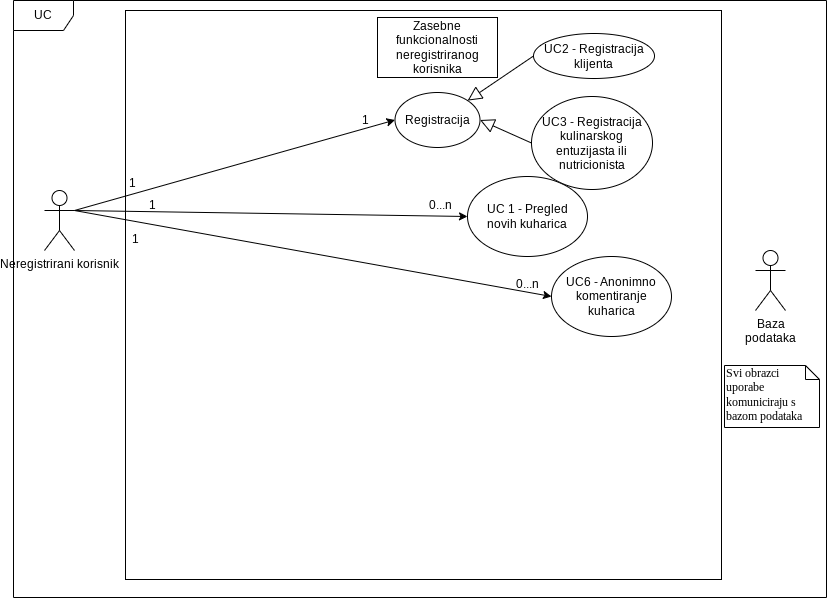
\includegraphics[scale=0.5]{dijagrami/dijagram-obrazaca-uporabe-neregistriranog-korisnika.png}
						\caption{Dijagram obrasca uporabe za neregistriranog korisnika}
						\label{fig:uc-neregistrirani}
					\end{figure}
					\begin{figure}[H]
						\centering
						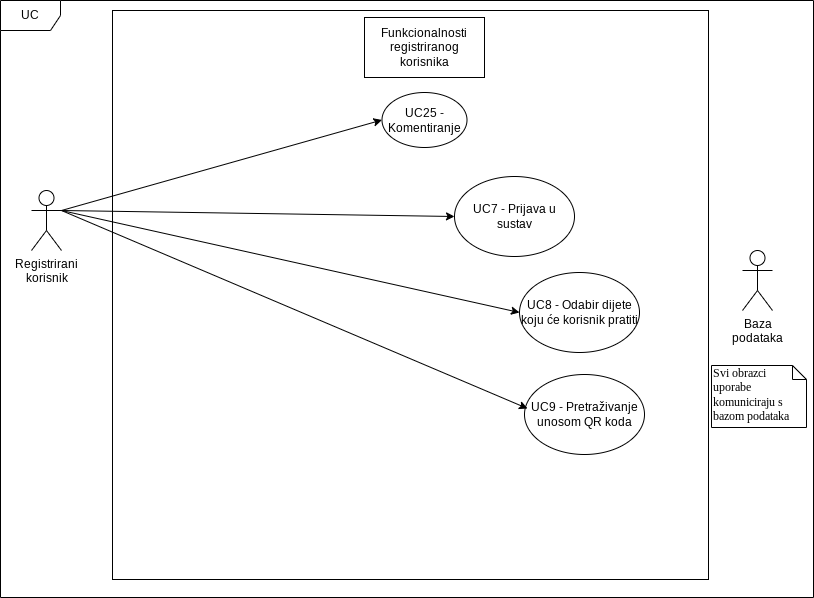
\includegraphics[scale=0.5]{dijagrami/dijagram-obrazaca-uporabe-registriranog-korisnika.png}
						\caption{Dijagram obrasca uporabe za registriranog korisnika}
						\label{fig:uc-registrirani}
					\end{figure} 
					\begin{figure}[H]
						\centering
						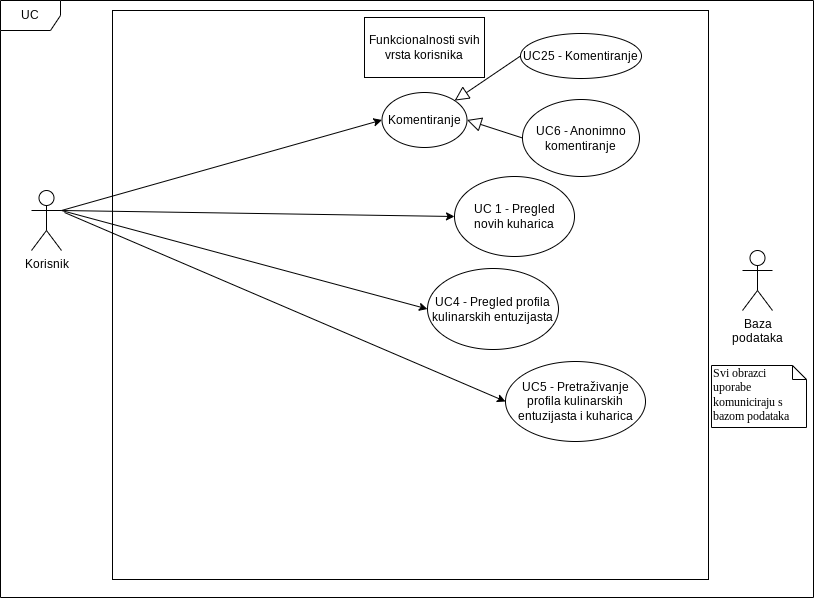
\includegraphics[scale=0.5]{dijagrami/dijagram-obrazaca-uporabe-za-sve-korisnike.png}
						\caption{Dijagram obrasca uporabe zajedničkog za sve korisnike}
						\label{fig:uc-svi-korisnici}
					\end{figure}
					\begin{figure}[H]
						\centering
						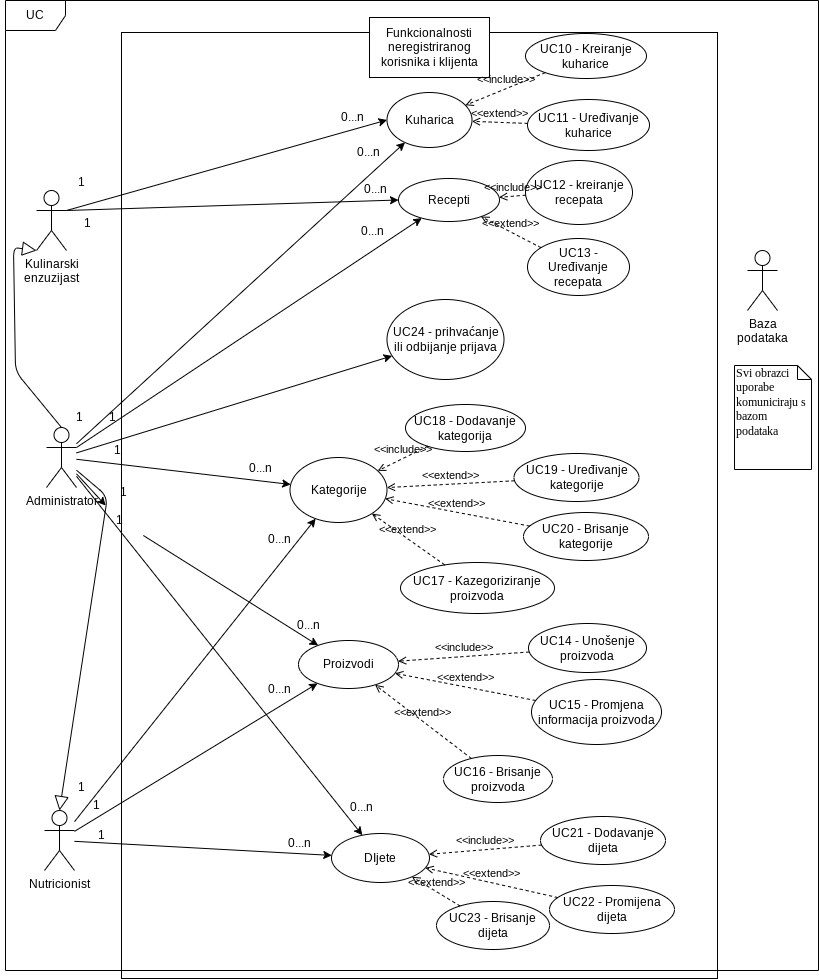
\includegraphics[scale=0.5]{dijagrami/dijagram-obrazaca-uporabe-kulinarskog-entuzijasta-i-nutricionista.png}
						\caption{Dijagram obrasca uporabe za kulinarskog entuzijasta i nutricionista}
						\label{fig:uc-kulinarski-i-nutricionist}
					\end{figure}
%					\textit{Prikazati odnos aktora i obrazaca uporabe odgovarajućim UML dijagramom. Nije nužno nacrtati sve na jednom dijagramu. Modelirati po razinama apstrakcije i skupovima srodnih funkcionalnosti.}

				\eject		
				
			\subsection{Sekvencijski dijagrami}
					\begin{figure}[H]
						\centering
						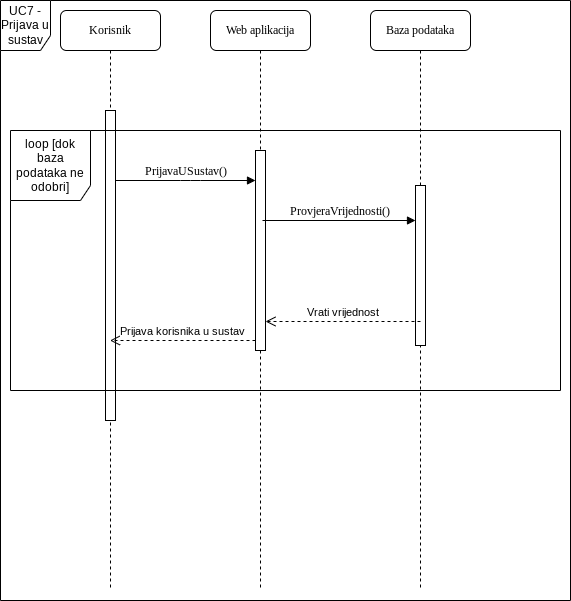
\includegraphics[scale=0.5]{dijagrami/sekvencijski-dijagram-prijave-u-sustav.png}
						\caption{Sekvencijski dijagram prijave u sustav}
						\label{fig:sekv-prijava}
					\end{figure}
					\subsubsection{Opis dijagrama}
						Korisnik u sučelju za prijavu u sustav upisuje potrebne podatke. Web aplikacija unesene podatke šalje bazi podataka. Baza podataka, nakon provjere postoji li par vrijednosti username - password među spremljenim vrijednostima, šalje poruku potvrde ili negacije postojanja para vrijednosti među podatcima. Web aplikacija nakon primanja potvrde dopušta prijavu, a nakon primanja dobijanja informira korisnika o neispravnosti podataka i ostaje u sučelju za prijavu gdje korisnik može ponoviti postupaks. 
					
					\begin{figure}[H]
						\centering
						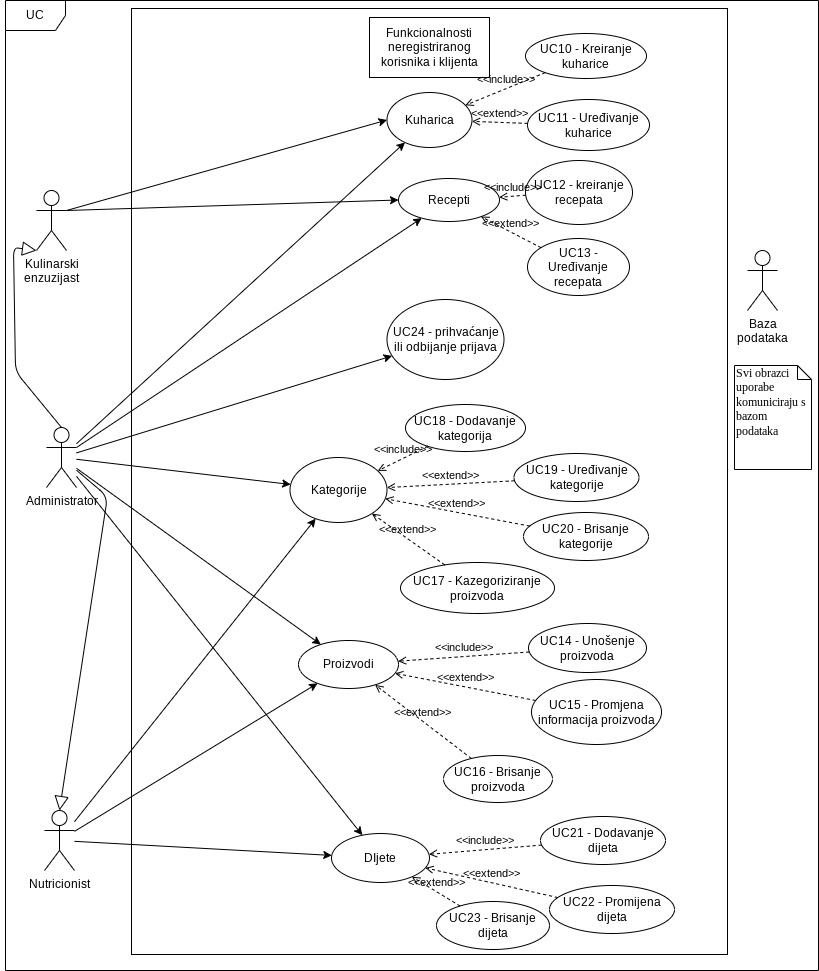
\includegraphics[scale=0.5]{dijagrami/sekvencijski-dijagram-registracije-nutricionista-i-kulinarskih-entuzijasta.png}
						\caption{Sekvencijski dijagram-registracije nutricionista i kulinarskih entuzijasta}
						\label{fig:sekv-registracija}
					\end{figure}
					\subsubsection{Opis dijagrama}
						Korisnik u sučelju za registraciju nutricionista ili kulinarskog entuzijasta unosi potrebne podatke. Nakon predaje registracije korisnik nastavlja koristiti web aplikaciju sa statusom klijenta. Web aplikacija podatke o registraciji šalje bazi podataka koja ih sprema. Nakon prijave administratora u sustav, baza podataka šalje podatke registracije web aplikaciji koja ih potom prikazuje administratoru. Administrator pregledava priložene informacije i odobrava ili odbija registraciju korisnika. Web aplikacija podatke o odluci  šalje bazi podataka koja bazirano na njima ima priliku promijeniti status korisnika. Nakon primanja podataka, baza podataka šalje informacije web aplikaciji koja prilaže informacije korisniku o uspješnoj registraciji ili o neuspješnoj registraciji i pruža korisniku priliku da izmijeni unesene podatke. 





%				\textbf{\textit{dio 1. revizije}}\\
%				
%				\textit{Nacrtati sekvencijske dijagrame koji modeliraju najvažnije dijelove sustava (max. 4 dijagrama). Ukoliko postoji nedoumica oko odabira, razjasniti s asistentom. Uz svaki dijagram napisati detaljni opis dijagrama.}
				\eject
	
		\section{Ostali zahtjevi}
			\begin{packed_item}
				\item Potrebno je omogućiti rad više korisnika u isto vrijeme.
				\item Sustav mora biti implementiran web aplikacijom
				\item Osjetljivi podatci poput lozinki moraju biti pohranjeni na adekvatan način, to jest kriptirani
				\item Korisničko sučelje mora biti otporno na pogreške tijekom korištenja
				\item Sustav mora biti javno dostupan putem web domene 
				\item Promet koji razmjenjuju klijent i poslužitelj mora biti zaštićen protokolom HTTPS
				\item Aplikacija mora biti razvijena koristeći objektno-orijentiranu paradigmu
			\end{packed_item}
%			\textbf{\textit{dio 1. revizije}}\\
%		 
%			 \textit{Nefunkcionalni zahtjevi i zahtjevi domene primjene dopunjuju funkcionalne zahtjeve. Oni opisuju \textbf{kako se sustav treba ponašati} i koja \textbf{ograničenja} treba poštivati (performanse, korisničko iskustvo, pouzdanost, standardi kvalitete, sigurnost...). Primjeri takvih zahtjeva u Vašem projektu mogu biti: podržani jezici korisničkog sučelja, vrijeme odziva, najveći mogući podržani broj korisnika, podržane web/mobilne platforme, razina zaštite (protokoli komunikacije, kriptiranje...)... Svaki takav zahtjev potrebno je navesti u jednoj ili dvije rečenice.}
			 
			 
			 
	
	\chapter{Arhitektura i dizajn sustava}
\setlength{\headheight}{14.49998pt}		
		%\textbf{\textit{dio 1. revizije}}\\

		%\textit{ Potrebno je opisati stil arhitekture te identificirati: podsustave, preslikavanje na radnu platformu, spremišta podataka, mrežne protokole, globalni upravljački tok i sklopovsko-programske zahtjeve. Po točkama razraditi i popratiti odgovarajućim skicama:}
	%\begin{itemize}
		%\item 	\textit{izbor arhitekture temeljem principa oblikovanja pokazanih na predavanjima (objasniti zašto ste baš odabrali takvu arhitekturu)}
		%\item 	\textit{organizaciju sustava s najviše razine apstrakcije (npr. klijent-poslužitelj, baza podataka, datotečni sustav, grafičko sučelje)}
		%\item 	\textit{organizaciju aplikacije (npr. slojevi frontend i backend, MVC arhitektura) }
	%\end{itemize}

Stil arhitekture korišten za izradu ovog sustava je mješavina objektno usmjerenog arhitekturnog stila, te stila Model-Pogled-Nadglednik (MVC), kombinirajući prednosti obje arhitekture dok se istovremeno poništavaju njihovi nedostaci. Korisničko je sučelje izdvojeno od ostatka sustava, dok je općenit pristup rješenju objektno orijentiran. Sustav je podijeljen na tri glavna, manja podsustava:
\begin{itemize}
\item Bazu podataka
\item Obradu podataka (backend)
\item Korisničko sučelje (frontend)
\end{itemize}
Podsustav za obradu podataka jedini surađuje sa bazom, a podaci se ne spremaju nigdje osim u bazu. Korisničko sučelje pak sve podatke dobiva iz podsustava za obradu te se time osigurava integritet i dosljednost sustava.
Podsustav za obradu i korisničko sučelje komuniciraju putem HTTPS protokola, dok se sa bazom komunicira upitima prema njoj.

				
		\section{Baza podataka}
			
			%\textbf{\textit{dio 1. revizije}}\\
			
		%\textit{Potrebno je opisati koju vrstu i implementaciju baze podataka ste odabrali, glavne komponente od kojih se sastoji i slično.}
Za pohranjivanje svih potrebnih informacija o korisnicima i njihovim aktivnostima u aplikaciji koristimo relacijski model baze poodataka. Glavna komponenta relacijske baze podataka je relacija. Relacija je imenovana dvodimenzinalna tablica koja predtavlja neki entitet čije informacije želimo preslikati u bazu podataka. Stupci tablice predstavljaju atribute entiteta, a redovi su n-torke tih atributa koji predstavljaju jednu instancu tog entiteta. Baza podataka ove aplikacije sastoji se od entiteta:
\begin{itemize}
\item Korisnik
\item PrivilegiraniKorisnik
\item Recept
\item Korak
\item PotrebniSastojci
\item Proizvod
\item OznakeProivoda
\item DodatneOznake
\item Kuharica
\item KuharicaSadržiRecept
\item KomentarKuharica
\item KomantarRecept
\item Konzumirao
\item Dijeta
\item Restrikcija
\end{itemize}

			\subsection{Opis tablica}
			

				%\textit{Svaku tablicu je potrebno opisati po zadanom predlošku. Lijevo se nalazi točno ime varijable u bazi podataka, u sredini se nalazi tip podataka, a desno se nalazi opis varijable. Svjetlozelenom bojom označite primarni ključ. Svjetlo plavom označite strani ključ}
		
				
\textbf{Slike}- Entitet slike sadrži sve slike koje su potrebne u opisu svih dalje navedenih entiteta
\begin{longtblr}[
					label=none,
					entry=none
					]{
						width = \textwidth,
						colspec={|X[6,l]|X[6, l]|X[20, l]|}, 
						rowhead = 1,
					}
					\hline \SetCell[c=3]{c}{\textbf{Slike}} \\ \hline[3pt]
					\SetCell{LightGreen}IDslika & INT & ID slike \\ \hline
					Slika & BYTEA & Binarni zapis slike \\ \hline
				\end{longtblr}

\textbf{Korisnik}- opisuje sve korisnike koji su registrirani na stranici. Entitet korisnik ima osnovne informacije  o korisnicima
t.j. ima atribute Korisničko ime(Posebno za svakog korisnika), lozinku, salt koji je nasumično generiran dodatak lozinki kako bi se postigla veća sigurnost pri korištenju hash funkcije, ime i prezime, te koji je tip korisnika(normalni korisnik, kulinarski entuzijast ili neutricionist) preko adtributa razinaprivilegije.
Za pohranu dodatnih podataka koje trebaju imati kulinarski entuzijast i nutricionist, potreban je slabi entitet PrivilegiraniKorisnik.
Taj entitet ima atribute email, biografija, ID slike(1,1 veza), te korisničko ime(identifikacijska 1,1 veza)
Korisnik je povezan sa dijetom koju prati preko imena dijete(N,1 veza).
Korisnici mogu pratiti druge korisnike, što je zapisano u zasebnoj tablici.
\begin{longtblr}[
					label=none,
					entry=none
					]{
						width = \textwidth,
						colspec={|X[8,l]|X[6, l]|X[18, l]|}, 
						rowhead = 1,
					}
					\hline \SetCell[c=3]{c}{\textbf{Korisnik}}	 \\ \hline[3pt]
					\SetCell{LightGreen}KorisnickoIme & VARCHAR & Korisničko ime korisnika \\ \hline
					Lozinka & VARCHAR & Lozinka korisnika \\ \hline 
					Salt & BYTEA & Dodatak lozinki \\ \hline 
					Ime & VARCHAR & Ime korisnika \\ \hline
					Prezime & VARCHAR & Prezime korisnika \\ \hline
					RazinaPrivilegije& INT & Razina/tip korisnika\\ \hline 
					\SetCell{LightBlue} ImeDijeta & VARCHAR & Ime dijete koju korisnik prati \\ \hline 
				\end{longtblr}

				\begin{longtblr}[
					label=none,
					entry=none
					]{
						width = \textwidth,
						colspec={|X[6,l]|X[6, l]|X[20, l]|}, 
						rowhead = 1,
					}
					\hline \SetCell[c=3]{c}{\textbf{PrivilegiraniKorisnik}}	 \\ \hline[3pt]
					\SetCell{LightGreen}KorisnickoIme & VARCHAR & Korisničko ime korisnika \\ \hline
					Biografija & VARCHAR & Biografija korisnika \\ \hline
					Email & VARCHAR & E-mail adresa korisnika \\ \hline
					\SetCell{LightBlue} IDslika & INT & ID slike korisnika \\ \hline 
				\end{longtblr}


				\begin{longtblr}[
					label=none,
					entry=none
					]{
						width = \textwidth,
						colspec={|X[7,l]|X[6, l]|X[19, l]|}, 
						rowhead = 1,
					}
					\hline \SetCell[c=3]{c}{\textbf{PratiKorisnika}} \\ \hline[3pt]
					\SetCell{LightBlue}KorisnickoIme\_1 & VARCHAR & Korisnik koji prati \\ \hline
					\SetCell{LightBlue}KorisnickoIme\_2 & VARCHAR & Korisnik koji je praćen \\ \hline
				\end{longtblr}


\textbf{Recept}- sadrži informacije o receptima . Sam entitet recept ima atribute ID recepta, datum izrade,
vrijeme pripreme i veličine porcija. Recept je povezan sa entitetom entuzijast(N,1 veza, predstavlja autora recepta). Svaki recept je podijeljen na korake, te su oni opisani posebnim entitetom. U N,N vezi sa entitetom Kuharica(veza je opisana entitetom Sadrži) i u N,N vezi 
s entitetom korisnik na dva načina(entiteti KomentarRecept i Konzumirao) 
\begin{longtblr}[
					label=none,
					entry=none
					]{
						width = \textwidth,
						colspec={|X[7,l]|X[6, l]|X[19, l]|}, 
						rowhead = 1,
					}
					\hline \SetCell[c=3]{c}{\textbf{Recept}}	 \\ \hline[3pt]
					\SetCell{LightGreen}IDrecept & INT & ID recepta \\ \hline
					ImeRecept & VARCHAR & Ime recepta \\ \hline
					VelicinaPorcija & INT & Veličina porcije \\ \hline
					VrijemePripreme & TIME & Vrijeme pripreme jela \\ \hline
					DatumIzrade & DATE & Datum izrade recepta \\ \hline
					\SetCell{LightBlue} KorisnickoIme & VARCHAR & Autor recepta \\ \hline 
				\end{longtblr}



\textbf{Korak}- sadrži sve informacije o pojedinim koracima nekog recepta. Ima atribute opis slike i opis koraka. Povezan je sa receptom
preko ID-a recepta(N,1 veza), i sa slikom preko ID-a slike(1,1 veza).
\begin{longtblr}[
					label=none,
					entry=none
					]{
						width = \textwidth,
						colspec={|X[6,l]|X[6, l]|X[20, l]|}, 
						rowhead = 1,
					}
					\hline \SetCell[c=3]{c}{\textbf{Korak}} \\ \hline[3pt]
					\SetCell{LightBlue}IDslika & INT & ID slike koraka \\ \hline
					\SetCell{LightBlue}IDrecept & INT & ID recepta \\ \hline
					OpisSl & VARCHAR & Opis slike \\ \hline 
					OpisKorak & VARCHAR & Opis koraka \\ \hline
				\end{longtblr}
\textbf{Potrebni sastojci}- opisuje N,N vezu između entiteta recept i proizvod. Svaka instanca ovog entiteta predstavlja jedan od potrebnih
sastojaka za neki recept.
Povezan je s receptom preko ID-a recepta(N,1 veza)
\begin{longtblr}[
					label=none,
					entry=none
					]{
						width = \textwidth,
						colspec={|X[6,l]|X[6, l]|X[20, l]|}, 
						rowhead = 1,
					}
					\hline \SetCell[c=3]{c}{\textbf{PotrebniSastojci}} \\ \hline[3pt]
					\SetCell{LightBlue}IDrecept & INT & Recept kojem čiji je sastojak \\ \hline
					\SetCell{LightBlue}IDproizvod & INT & proizvod koji je sastojak \\ \hline
					Kolicina & NUMERICAL & Količina proizvoda u gramima \\ \hline
				\end{longtblr}
 
\textbf{Proizvod}- Sadrži sve potrebne informacije o proizvodima. ima atribute ID proizvoda, ime proizvoda, energija, masnoće, zasićene masne kiseline, ugljikohidrati, šećeri, bjelančevine, sol i slika proizvoda(1,1 veza sa Slike). Svaki proizvod može imati jednu ili više posebnih oznaka(N,N veza sa entitetom DodatneOznake koja je opisana entitetom OznakeProizvoda)
\begin{longtblr}[
					label=none,
					entry=none
					]{
						width = \textwidth,
						colspec={|X[7,l]|X[6, l]|X[19, l]|}, 
						rowhead = 1,
					}
					\hline \SetCell[c=3]{c}{\textbf{Proizvod}}	 \\ \hline[3pt]
					\SetCell{LightGreen}IDproizvod & INT & Identifikacijski broj proizvoda \\ \hline
					MasaPr & NUMERICAL & Masa proizvoda u gramima \\ \hline 
					ImeProizvod & VARCHAR & Ime proizvoda \\ \hline
					EnergijaPr & NUMERICAL & Količina energije na 100 grama u kilodžulima \\ \hline 
					MasnocePr & NUMERICAL & Količina masti na 100 grama u gramima \\ \hline
					ZMKiselinePr & NUMERICAL & Količina zasićenih masnih kiselina na 100 grama u gramima \\ \hline
					UgljikohidratiPr & NUMERICAL & Količina ugljikohidrata na 100 grama u gramima \\ \hline
					SeceriPr & NUMERICAL & Količina šećera na 100 grama u gramima \\ \hline
					BjelancevinePr & NUMERICAL & Količina bjelančevina na 100 grama u gramima \\ \hline
					SolPr & NUMERICAL & Količina soli na 100 grama u gramima \\ \hline 
					\SetCell{LightBlue} IDslika	& INT & ID slika proizvoda \\ \hline 
				\end{longtblr}
\begin{longtblr}[
					label=none,
					entry=none
					]{
						width = \textwidth,
						colspec={|X[6,l]|X[6, l]|X[20, l]|}, 
						rowhead = 1,
					}
					\hline \SetCell[c=3]{c}{\textbf{OznakeProizvoda}} \\ \hline[3pt]
					\SetCell{LightBlue}IDproizvod & INT & ID proizvoda \\ \hline
					\SetCell{LightBlue}IDOzn & INT & ID dodatne oznake proizvoda \\ \hline
				\end{longtblr}

\textbf{DodatneOznake}- Opisuje dodatne oznake koje neki proizvod može imati. U N,N vezi s entitetom Proizvod
koja je opisana entitetom OznakeProizvoda. Također u N,N vezi s Dijeta koja je opisana entitetom Restrikcija
\begin{longtblr}[
					label=none,
					entry=none
					]{
						width = \textwidth,
						colspec={|X[6,l]|X[6, l]|X[20, l]|}, 
						rowhead = 1,
					}
					\hline \SetCell[c=3]{c}{\textbf{DodatneOznake}} \\ \hline[3pt]
					\SetCell{LightBlue}IDOzn & INT & ID dodatne oznake \\ \hline
					OpisOzn & VARCHAR & Opis dodatne oznake \\ \hline
				\end{longtblr}

\textbf{Kuharica}- Sadrži informacije o kuharicama. Atributi su ID, tema, naslov, datum izrade i korisničko ime autora(N,1 veza sa Entuzijast). 
Entitet je u N,N vezi s Korisnik(pisan entitetom 
KomentarKuharica). Svaka kuharica je is karakterizirana listom recepata koje sadrži(N,N veza s Recept koja je opisana entitetom KuharicaSadrziRecept)
\begin{longtblr}[
					label=none,
					entry=none
					]{
						width = \textwidth,
						colspec={|X[6,l]|X[6, l]|X[20, l]|}, 
						rowhead = 1,
					}
					\hline \SetCell[c=3]{c}{\textbf{Kuharica}} \\ \hline[3pt]
					\SetCell{LightGreen}IDkuharica & INT & ID recepta \\ \hline
					Tema & VARCHAR & Tema kuharice \\ \hline
					Naslov & VARCHAR & Naslov kuharice \\ \hline
					DatumIzrade & DATE & Datum izrade recepta \\ \hline
					\SetCell{LightBlue} KorisnickoIme & VARCHAR & Autor kuharice \\ \hline 
				\end{longtblr}
\begin{longtblr}[
					label=none,
					entry=none
					]{
						width = \textwidth,
						colspec={|X[6,l]|X[6, l]|X[20, l]|}, 
						rowhead = 1,
					}
					\hline \SetCell[c=3]{c}{\textbf{KuharicaSadrziRecept}} \\ \hline[3pt]
					\SetCell{LightBlue}IDrecept & INT & Recept u kuharici \\ \hline
					\SetCell{LightBlue}IDKuharica & INT & Kuharica koja sadrži recept \\ \hline
				\end{longtblr}
\textbf{KomentarRecept}- opisuje N,N vezu između korisnika i recepta koja predstavlja recenziju korisnika za neki recept. Atributi su ID komentara na receptu, korisničko ime(N,1 veza s korisnik), ID recepta(N,1 veza s
recept), ocjena koju je korisnik ostavio, komentar korisnika, te odgovor od autora recepta(ako ga ima).
\begin{longtblr}[
					label=none,
					entry=none
					]{
						width = \textwidth,
						colspec={|X[10,l]|X[6, l]|X[16, l]|}, 
						rowhead = 1,
					}
					\hline \SetCell[c=3]{c}{\textbf{KomentarRecept}} \\ \hline[3pt]
					\SetCell{LightGreen}IDKomentarRecept & INT & ID Komentara za recepte \\ \hline
					\SetCell{LightBlue}KorisnickoIme & VARCHAR & Korisnicko ime autora komentara \\ \hline
					\SetCell{LightBlue}IDrecept & INT & ID recepta na kojem je komentar \\ \hline
					SadrzajKomentaraR & VARCHAR & Sadržaj komentara \\ \hline
					OdgovorNaKomentar & VARCHAR & Odgovar na komentar \\ \hline
					OcjenaR & INT & Ocjena recepta \\ \hline
				\end{longtblr}
\textbf{KomentarKuharica}-opisuje N,N vezu između korisnika i kuharice koja predstavlja recenziju korisnika za neku kuharicu.
 Atributi su ID komentara na kuharici, korisničko ime(N,1 veza s korisnik), ID kuharice(N,1 veza s
kuharica), ocjena koju je korisnik ostavio, komentar korisnika, te odgovor od autora kuharice(ako ga ima).
\begin{longtblr}[
					label=none,
					entry=none
					]{
						width = \textwidth,
						colspec={|X[10,l]|X[6, l]|X[16, l]|}, 
						rowhead = 1,
					}
					\hline \SetCell[c=3]{c}{\textbf{KomentarKuharica}} \\ \hline[3pt]
					\SetCell{LightGreen}IDKomentarKuharica & INT & ID Komentara za kuharice \\ \hline
					\SetCell{LightBlue}KorisnickoIme & VARCHAR & Korisničko ime autora \\ \hline
					\SetCell{LightBlue}IDkuharica & INT & ID komentirane kuharice \\ \hline
					SadrzajKomentaraK & VARCHAR & Sadržaj komentara \\ \hline
					OdgovorNaKomentarK & VARCHAR & Odgovor na komentar \\ \hline
					OcjenaK & INT & Ocjena kuharice \\ \hline 
				\end{longtblr}
\textbf{Konzumirao}- opisuje N,N vezu između korisnika i recepta koja označuje da je neki korisnik probao neki recept. Atributi su korisničko ime(N,1 veza s korisnik), ID recepta(N,1 veza srecept) te datum zapisa.
\begin{longtblr}[
					label=none,
					entry=none
					]{
						width = \textwidth,
						colspec={|X[10,l]|X[6, l]|X[16, l]|}, 
						rowhead = 1,
					}
					\hline \SetCell[c=3]{c}{\textbf{Konzumirao}} \\ \hline[3pt]
					\SetCell{LightBlue}KorisnickoIme & VARCHAR & Korisničko ime \\ \hline
					\SetCell{LightBlue}IDrecept & INT & ID konzumiranog recepta \\ \hline
					Datum & DATE & Datum konzumiranja \\ \hline
				\end{longtblr}
\textbf{Dijeta}- Sadrži sve informacije o dijetama. Atributi su ime, opis, minimalne i maksimalne vrijednosti nutrijenata po proizvodu koje dopušta dijeta, te maksimalni dnevni unos tih nutrijenata(nutrijenti su isti oni kao i u opisu entiteta proizvod :energija, masnoće, zasićene masne kiseline, ugljikohidrati, šećeri, bjelančevine i sol). Atributi spomenuti nakon opisa služe kako bi se omogučilo filtritanje recepata korisniku s obzirom na to dali  taj recept zadovoljava parametre neke dijete. U N,N vezi je s entitetom 
DodatneOznake(veza je opisana entitetom Restrikcija i predstavlja restrikcije dijete na proizvode s tim oznakama) 
\begin{longtblr}[
					label=none,
					entry=none
					]{
						width = \textwidth,
						colspec={|X[11,l]|X[6, l]|X[16, l]|}, 
						rowhead = 1,
					}
					\hline \SetCell[c=3]{c}{\textbf{Dijeta}}	 \\ \hline[3pt]
					\SetCell{LightGreen}ImeDijeta & VARCHAR & Ime dijete \\ \hline
					Opis & VARCHAR & Opis dijete \\ \hline
					MinEnergija & NUMERICAL & Minimalna količina energije u receptu \\ \hline 
					MaxEnergija & NUMERICAL & Maksimalna količina energije u receptu \\ \hline 
					MinMasnoce & NUMERICAL & Minimalna količina masti u receptu \\ \hline
					MaxMasnoce & NUMERICAL & Maksimalna količina masti u receptu \\ \hline
					MinZMKiseline & NUMERICAL & Minimalna količina zasićenih masnih kiselina u receptu \\ \hline
					MaxZMKiseline & NUMERICAL & Maksimalna količina zasićenih masnih kiselina u receptu \\ \hline
					MinUgljikohidrati & NUMERICAL & Minimalna količina ugljikohidrata u receptu \\ \hline
					MaxUgljikohidrati & NUMERICAL & Maksimalna količina ugljikohidrata u receptu \\ \hline
					MinSeceri & NUMERICAL & Minimalna količina šećera u receptu \\ \hline
					MaksSeceri & NUMERICAL & Maksimalna količina šećera u receptu \\ \hline
					MinBjelancevine & NUMERICAL & Minimalna količina bjelančevina u receptu \\ \hline
					MaxBjelancevine & NUMERICAL & Maksimalna količina bjelančevina u receptu \\ \hline
					MinSol & NUMERICAL & Minimalna količina soli u receptu \\ \hline
					MaxSol & NUMERICAL & Maksimalna količina soli u receptu \\ \hline
					DnevniMaxEnergija & NUMERICAL & Dnevna maksimalna količina energije \\ \hline 
					DnevniMaxMasnoce & NUMERICAL & Dnevna maksimalna količina masti \\ \hline
					DnevniMaxZMKiseline & NUMERICAL & Dnevna maksimalna količina zasićenih masnih kiselina \\ \hline
					DnevniMaxUgljikohidrati & NUMERICAL & Dnevna maksimalna količina ugljikohidrata \\ \hline
					DnevniMaksSeceri & NUMERICAL & Dnevna maksimalna količina šećera \\ \hline
					DnevniMaxBjelancevine & NUMERICAL & Dnevna maksimalna količina bjelančevina \\ \hline
					DnevniMaxSol & NUMERICAL & Dnevna maksimalna količina soli \\ \hline
				\end{longtblr}			
\begin{longtblr}[
					label=none,
					entry=none
					]{
						width = \textwidth,
						colspec={|X[6,l]|X[6, l]|X[20, l]|}, 
						rowhead = 1,
					}
					\hline \SetCell[c=3]{c}{\textbf{Restrikcija}} \\ \hline[3pt]
					\SetCell{LightBlue}ImeDijeta & VARCHAR & Dijeta koja ima restrikciju \\ \hline
					\SetCell{LightBlue}IDOzn & INT & Dodatna oznaka na kojoj je restrikcija \\ \hline
				\end{longtblr}







\subsection{Dijagram baze podataka}
				%\textit{ U ovom potpoglavlju potrebno je umetnuti dijagram baze podataka. Primarni i strani ključevi moraju biti označeni, a tablice povezane. Bazu podataka je potrebno normalizirati. Podsjetite se kolegija "Baze podataka".}
			\begin{figure}[H]
					\centering
					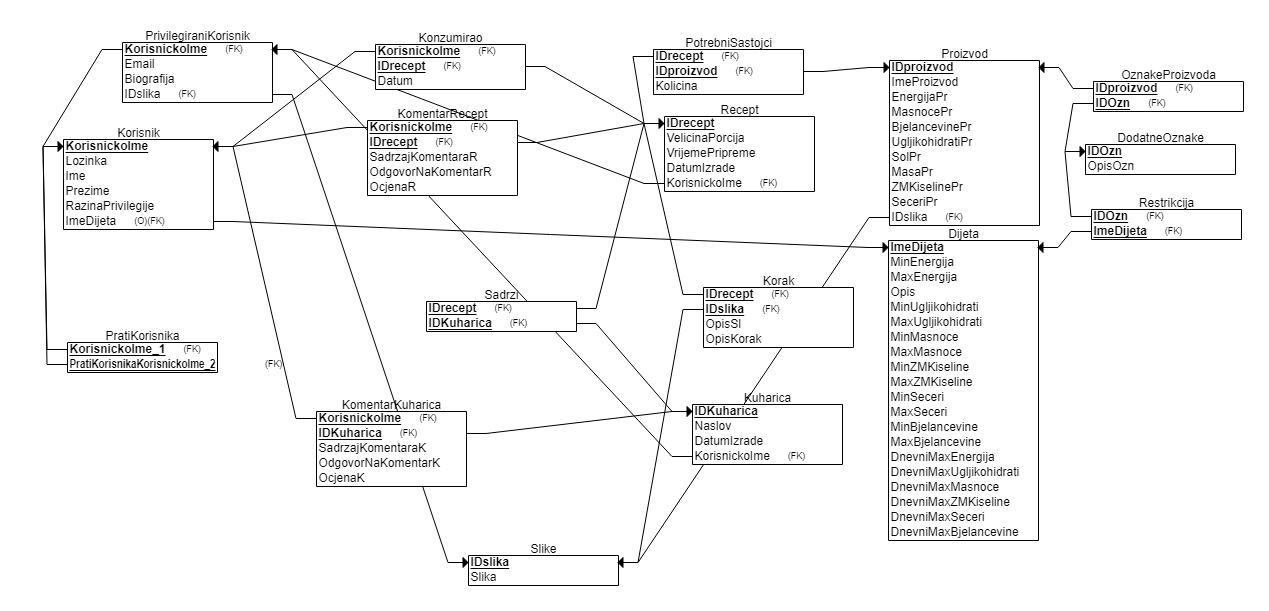
\includegraphics[scale=0.4]{slike/REL-model-baze.png}
					\caption{Relacijska shema baze podataka}
					\label{fig:REL-model-baze}
				\end{figure} 
			\eject
			
			
		\section{Dijagram razreda}
			\begin{figure}[H]
				\centering
				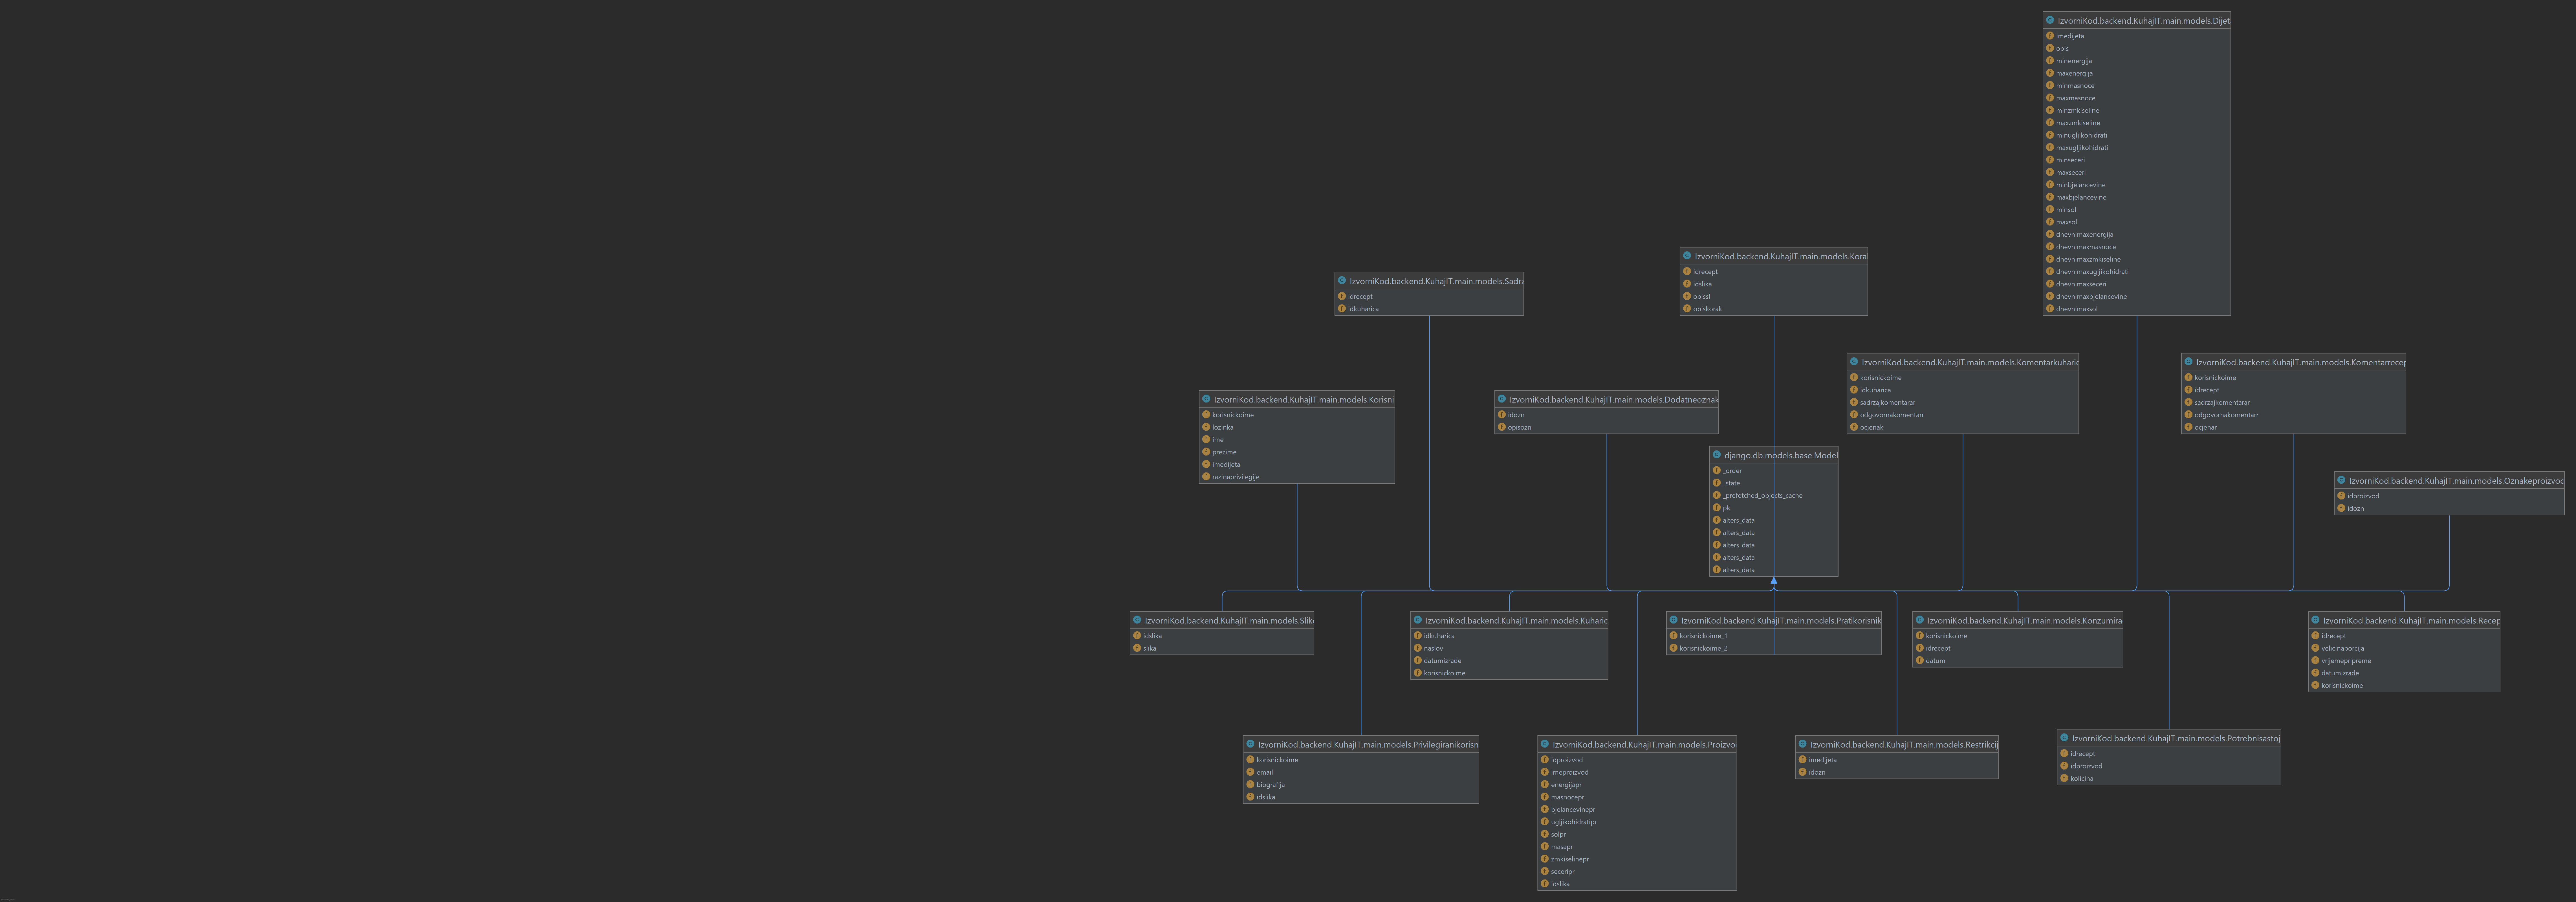
\includegraphics[scale=0.08]{dijagrami/dijagram-klasa.png}
				\caption{dijagram klasa}
				\label{fig:klase}
			\end{figure}
			%\textit{Potrebno je priložiti dijagram razreda s pripadajućim opisom. Zbog preglednosti je moguće dijagram razlomiti na više njih, ali moraju biti grupirani prema sličnim razinama apstrakcije i srodnim funkcionalnostima.}\\
			
			%\textbf{\textit{dio 1. revizije}}\\
			
			\textit{Prilikom prve predaje projekta, potrebno je priložiti potpuno razrađen dijagram razreda vezan uz \textbf{generičku funkcionalnost} sustava. Ostale funkcionalnosti trebaju biti idejno razrađene u dijagramu sa sljedećim komponentama: nazivi razreda, nazivi metoda i vrste pristupa metodama (npr. javni, zaštićeni), nazivi atributa razreda, veze i odnosi između razreda.}\\
			
			\textbf{\textit{dio 2. revizije}}\\			
			
			\textit{Prilikom druge predaje projekta dijagram razreda i opisi moraju odgovarati stvarnom stanju implementacije}
			
			
			
			\eject
		
		\section{Dijagram stanja}
			
			
			%\textbf{\textit{dio 2. revizije}}\\
			
			%\textit{Potrebno je priložiti dijagram stanja i opisati ga. Dovoljan je jedan dijagram stanja koji prikazuje \textbf{značajan dio funkcionalnosti} sustava. Na primjer, stanja korisničkog sučelja i tijek korištenja neke ključne funkcionalnosti jesu značajan dio sustava, a registracija i prijava nisu. }
			
			\begin{figure}[H]
				\centering
				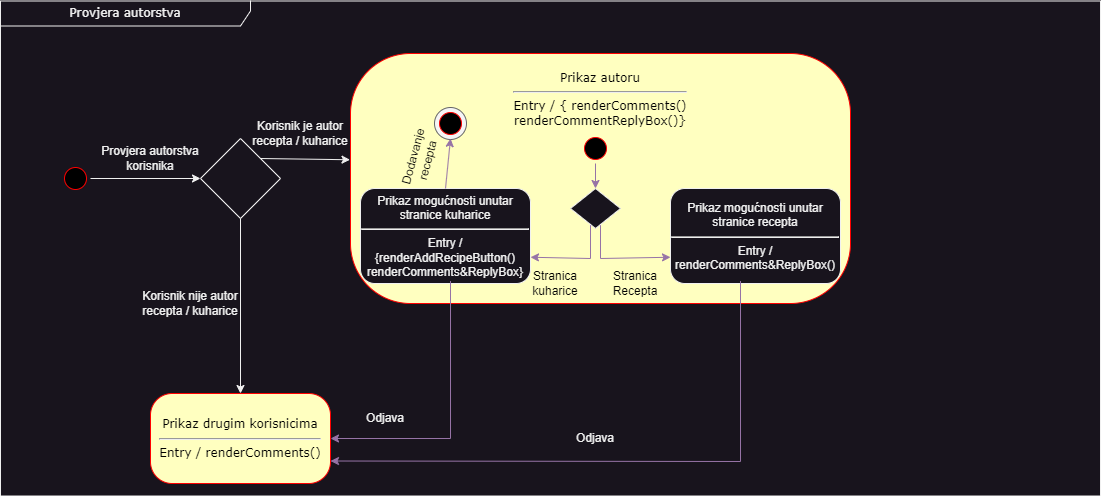
\includegraphics[scale=0.35]{dijagrami/DijagramStanjaProvjereAutorstva.png}
				\caption{dijagram stanja provjere autorstva}
				\label{fig:autorstvo}
			\end{figure}
			
			
			\eject 
		
		\section{Dijagram aktivnosti}
			
			\textbf{\textit{dio 2. revizije}}\\
			
			 \textit{Potrebno je priložiti dijagram aktivnosti s pripadajućim opisom. Dijagram aktivnosti treba prikazivati značajan dio sustava.}
			
			\eject
		\section{Dijagram komponenti}
		
			\textbf{\textit{dio 2. revizije}}\\
		
			 \textit{Potrebno je priložiti dijagram komponenti s pripadajućim opisom. Dijagram komponenti treba prikazivati strukturu cijele aplikacije.}

	\chapter{Implementacija i korisničko sučelje}
		
		
		\section{Korištene tehnologije i alati}
		
			%\textbf{\textit{dio 2. revizije}}
			
			 %\textit{Detaljno navesti sve tehnologije i alate koji su primijenjeni pri izradi dokumentacije i aplikacije. Ukratko ih opisati, te navesti njihovo značenje i mjesto primjene. Za svaki navedeni alat i tehnologiju je potrebno \textbf{navesti internet poveznicu} gdje se mogu preuzeti ili više saznati o njima}.
			 \subsection{Tehnologije koje čine aplikaciju}
			 	Aplikacija ima  \href{https://www.djangoproject.com/}{Django} backend i \href{https://react.dev/}{React} frontend te za bazu podataka koristi \href{https://www.postgresql.org/}{PostgreSQL}. Django je web framework za Python koji je dostatan za izradu cijelih web aplikacija jer obuhvaća izradu sučelja putem HTML-a i CSS-a, komunikaciju s bazom podataka i backend logiku u jeziku Python. On s bazom podataka komunicira tako da preslikava Python objekte na bazu (takvi sustavi se još zovu ORM, kratica od Object Relational Mapping). Komunikacija s PostgreSQL bazom podataka se u Django-u ostvaruje korištenjem Python modula \href{https://pypi.org/project/psycopg2/}{psycopg2}. koji omogućuje spajanje na bazu podataka, njenu administraciju te slanje SQL upita poslužitelju baze podataka. To je ujedno i najkorišteniji Python modul za PostgreSQL, a tu je naveden jer ga eksplicitno koristimo u dijelovima aplikacije koji trebaju izvršiti velike upite na bazi podataka. Pri eksplicitnom komuniciranju s bazom, morali smo paziti da koristimo iste module kao i Django, kako ne bi nastali problemi s bazom. Naš tim je odlučio frontend odraditi u React frameworku, a s Django-om odraditi backend i komunikaciju s bazom. React i Django su u aplikaciji spojeni tehnologijom \href{https://www.django-rest-framework.org/}{Django REST framework}, koja omogućuje da oni komuniciraju međusobno. React je frontend web framework koji omogućuje izgradnju web sučelja korištenjem HTML-a, CSS-a i skriptnog jezika Javascript. React-om se najčešće izrađuju web sučelja, ali je moguće izraditi i takozvane desktop aplikacije koristeći tehnologije kao što je Electron. U tom slučaju se React aplikacija izvršava na instanci preglednika Google Chrome te je oblikovana da se ponaša kao ostale desktop aplikacije.
			
			\subsection{Tehnologije za komunikaciju s članovima tima}
				Za komunikaciju među članovima tima smo uglavnom koristili platforme Whatsapp i Discord te u manjem omjeru platforme Telegram i Element. Platformu MS Teams nismo koristili za komunikaciju među članovima tima jer ne podržava dobro preglednik Firefox i desktop aplikacija za operacijski sustav Linux je spora i nespretna za korištenje. Tri člana koriste Linux, a od toga dva imaju samo Linux na računalima. Stoga nam je bitno da svi alati podržavaju i Windows i Linux te da su na oba sustava iskoristivi u jednakom opsegu.
				
			\subsection{Tehnologije za pisanje dokumentacije}
				Pošto je zadano da dokumentaciju izrađujemo u LaTeX-u, a trebala nam distribucija koja podržava i Linux i Windows. odlučili smo se za \href{https://www.tug.org/texlive/}{TeX Live} jer postoji kao paket u repozitorijima modernih Linux distribucija. Za typesetting nam služi editor Texworks, koji je dio TeX Live distribucije. Odabir alata za uređivanje TEX datoteka je ostavljen članovima tima, a neki od odabranih uz TeXworks su: terminal editor \href{https://www.vim.org/}{Vim}, \href{https://code.visualstudio.com/}{Visual Studio Code} napravljen u Electron-u i \href{https://www.sublimetext.com/}{Sublime Text}.
			
			\subsection{Tehnologije za izradu popratnih sadržaja, odnosno dijagrama, grafika i prezentacija}
				Za izradu zadanih dijagrama najviše smo koristili \href{https://www.drawio.com/}{draw.io}, koji omogućuje laganu izradu dijagrama tehnikom drag and drop te sadrži sve potrebne elemente UML dijagrama. Pored toga još sadrži i dijagrame arhitekture strujnih krugova i mnoge druge tipove dijagrama. Međutim, postoje slučajevi kada dijagrame treba doraditi pa smo za to koristili \href{https://inkscape.org/}{Inkscape}, koji manipulira slike u SVG formatu. SVG je grafički format u kojem su slike predstavljene matematičkim formulama, a ne pikselima pa su stoga lako skalabilne bez da gube na razlučivosti. Za potrebe uređivanja slika koristili smo \href{https://www.gimp.org/}{GIMP}, a za skiciranje pri radu smo koristili program \href{https://krita.org/}{Krita}. Prezentacije izrađujemo alatom \href{https://www.libreoffice.org/}{Libreoffice Impress}.
				
			\subsection{Tehnologije za pisanje programskog koda}
				Programi opće namjene kojima smo pisali kod su: terminal editor \href{https://www.vim.org/}{Vim}, \href{https://code.visualstudio.com/}{Visual Studio Code} napravljen u Electron-u i \href{https://www.sublimetext.com/}{Sublime Text}. Pri pisanju Python-a, korišteno je razvojno okruženje \href{https://www.spyder-ide.org/}{Spyder}, a za provjeru frontenda preglednici \href{https://www.mozilla.org/en-US/firefox/new/}{Firefox} i \href{https://www.google.com/chrome/}{Google Chrome}. Koristili smo \href{https://www.pgadmin.org/download/}{pgAdmin4} za upravljanje bazom podataka.
				
			\subsection{Tehnologije vezane za sustav upravljanja inačicama}
				Osim programa Git, koristili smo i popratne alate da nam olakšaju rad na zajedničkom repozitoriju. Članovi na sustavu Linux su koristili \href{https://github.com/prati0100/git-gui/}{git-gui}, to je alat za upravljanje git commit-ovima s grafičkim sučeljem koji je dostupan i na Windows sustavima.	Uz njega je vezan alat gitk,	koji grafički prikazuje repozitorij, grane i povijest commit-ova. Također, on dopušta manipulaciju lokalnom povijesti repozitorija. Članovi na Windows sustavima su koristili \href{https://desktop.github.com/}{GitHub desktop}, koji ima grafičko sučelje. S obzirom da imamo članove na sustavima Linux i Windows koji surađuju, važno je podesiti alate tako da članovi na Windows sustavima u repozitorij šalju datoteke s Unix znakovima za kraj retka.
			\subsection{Sažetak}
				Većina odabranih alata ima javni izvorni kod s licencama koje dopuštaju korisniku da ih kopira, mijenja i distribuira, Izbor alata je posljedica iskustva voditelja projekta u radu s njima, a u namjeri da ostalim članovima može pomoći što više.
			\eject 
		
	
		\section{Ispitivanje programskog rješenja}
			
			%\textbf{\textit{dio 2. revizije}}\\
			
			 %\textit{U ovom poglavlju je potrebno opisati provedbu ispitivanja implementiranih funkcionalnosti na razini komponenti i na razini cijelog sustava s prikazom odabranih ispitnih slučajeva. Studenti trebaju ispitati temeljnu funkcionalnost i rubne uvjete.}
			Napomena: Ispitivanje nije implementirano zbog manjka članova koji rade u timu, što je odvuklo pozornost od testiranja. Međutim, u daljnjem tekstu je objašnjen proces testiranja Python koda.
			
			Za testiranje Python dijelova aplikacije namjeravali smo koristiti Python modul \href{https://docs.pytest.org/en/7.4.x/index.html}{pytest}. On nije dio standardnih modula pa ga je potrebno instalirati programom pip. Pytest bi nam omogućio jedinično testiranje, to jest vrijede li zadani logički izrazi. Također, pytest automatski detektira testne funkcije i module te ima detaljniji opis grešaka nego  standardni Python modul za testiranje, unittest. Sve testove pisali bi smo u Pythonu jer radimo sa Django-om preko kojeg komuniciramo s bazom podataka pa bi tako Python testovi pokrili i backend i bazu. React dio aplikacije nama dijelove koje smatramo vrijednima za testiranje ovim tipom testa jer se sastoji ili od statičkih dijelova (CSS i HTML) ili dijelova koji komuniciraju s Django-om, koji je zadužen za svu logiku. U slučaju da neki React dio ne radi, to ćemo vidjeti u pregledniku kao neželjeni prikaz elemenata grafičkog sučelja
			
			\subsection{Ispitivanje komponenti}
			%\textit{Potrebno je provesti ispitivanje jedinica (engl. unit testing) nad razredima koji implementiraju temeljne funkcionalnosti. Razraditi \textbf{minimalno 6 ispitnih slučajeva} u kojima će se ispitati redovni slučajevi, rubni uvjeti te izazivanje pogreške (engl. exception throwing). Poželjno je stvoriti i ispitni slučaj koji koristi funkcionalnosti koje nisu implementirane. Potrebno je priložiti izvorni kôd svih ispitnih slučajeva te prikaz rezultata izvođenja ispita u razvojnom okruženju (prolaz/pad ispita). }
				Ne postoji iz gore navedenih razloga.
			
			
			
			\subsection{Ispitivanje sustava}
			
			 %\textit{Potrebno je provesti i opisati ispitivanje sustava koristeći radni okvir Selenium\footnote{\url{https://www.seleniumhq.org/}}. Razraditi \textbf{minimalno 4 ispitna slučaja} u kojima će se ispitati redovni slučajevi, rubni uvjeti te poziv funkcionalnosti koja nije implementirana/izaziva pogrešku kako bi se vidjelo na koji način sustav reagira kada nešto nije u potpunosti ostvareno. Ispitni slučaj se treba sastojati od ulaza (npr. korisničko ime i lozinka), očekivanog izlaza ili rezultata, koraka ispitivanja i dobivenog izlaza ili rezultata.\\ }
			 	Ne postoji iz gore navedenih razloga.
			 %\textit{Izradu ispitnih slučajeva pomoću radnog okvira Selenium moguće je provesti pomoću jednog od sljedeća dva alata:}
			 %\begin{itemize}
			 	%\item \textit{dodatak za preglednik \textbf{Selenium IDE} - snimanje korisnikovih akcija radi automatskog ponavljanja ispita	}
			 	%\item \textit{\textbf{Selenium WebDriver} - podrška za pisanje ispita u jezicima Java, C\#, PHP koristeći posebno programsko sučelje.}
			 %\end{itemize}
		 	%\textit{Detalji o korištenju alata Selenium bit će prikazani na posebnom predavanju tijekom semestra.}
			
			\eject 
		
		
		\section{Dijagram razmještaja}
			
			\textbf{\textit{dio 2. revizije}}
			
			 \textit{Potrebno je umetnuti \textbf{specifikacijski} dijagram razmještaja i opisati ga. Moguće je umjesto specifikacijskog dijagrama razmještaja umetnuti dijagram razmještaja instanci, pod uvjetom da taj dijagram bolje opisuje neki važniji dio sustava.}
			
			\eject 
		
		\section{Upute za puštanje u pogon}
			
			%\textbf{\textit{dio 2. revizije}}\\
		
			 %\textit{U ovom poglavlju potrebno je dati upute za puštanje u pogon (engl. deployment) ostvarene aplikacije. Na primjer, za web aplikacije, opisati postupak kojim se od izvornog kôda dolazi do potpuno postavljene baze podataka i poslužitelja koji odgovara na upite korisnika. Za mobilnu aplikaciju, postupak kojim se aplikacija izgradi, te postavi na neku od trgovina. Za stolnu (engl. desktop) aplikaciju, postupak kojim se aplikacija instalira na računalo. Ukoliko mobilne i stolne aplikacije komuniciraju s poslužiteljem i/ili bazom podataka, opisati i postupak njihovog postavljanja. Pri izradi uputa preporučuje se \textbf{naglasiti korake instalacije uporabom natuknica} te koristiti što je više moguće \textbf{slike ekrana} (engl. screenshots) kako bi upute bile jasne i jednostavne za slijediti.}
			
			
			 %\textit{Dovršenu aplikaciju potrebno je pokrenuti na javno dostupnom poslužitelju. Studentima se preporuča korištenje neke od sljedećih besplatnih usluga: \href{https://aws.amazon.com/}{Amazon AWS}, \href{https://azure.microsoft.com/en-us/}{Microsoft Azure} ili \href{https://www.heroku.com/}{Heroku}. Mobilne aplikacije trebaju biti objavljene na F-Droid, Google Play ili Amazon App trgovini.}
			
			Upute podrazumijevaju da je slijedeće podešeno prije puštanja u pogon:
			\begin{itemize}
				\item Podešen PostgreSQL poslužitelj i pgadmin4 tako da mogu međusobno komunicirati
				\item Podešena instalacija Python-a 3.10 ili novijeg na razini sustava
				\item Podešena node.js instalacija s instaliranim upraviteljem paketa npm
				\item Podešen poslužitelj na način da je javno dostupan i komunikacija među portovima 3000 i 8000 nije onemogućena vatrozidom
			\end{itemize}	
			Napomena: Sljedeće upute će postaviti aplikaciju tako da se procesi Django, React i PostgreSQL izvršavaju na istom računalu
			
			Koraci:
			\begin{packed_enum}
				\item Otvorite naredbeni redak (cmd.exe ili terminal)
				\item Izvršite naredbu: git clone https://github.com/glatkobrasno/wall-e-zohari
				\item Komanda generira cijelo stablo direktorija, uključujući frontend (react) i backend (django) dijelove koda.
				Zatim se prebacite u backend direktorij koji je nastao prethodnom naredbom. Komanda: \\ cd  ./wall-e-zohari/IzvorniKod/backend/KuhajIT
				\item Napunite podatke u PostgreSQL bazu korištenjem pgadmin4 programom. Podatci za punjenje baze se nalaze u backend/KuhajIT direktoriju, KuhajITDatabase.sql. 
				\item Zatim se instalira i aktivira python virtualno okruženje, te instalitaju potrebni paketi komandama:
				\item[] \begin{packed_enum}
				    \item pip install virtualenv
				    \item virtualenv ../venv
     				\item ..\textbackslash venv\textbackslash Scripts\textbackslash activate.bat - u Windows okruženju
      				\item source ../venv/bin/activate - u Linux okruženju

				    \item pip install -r requirements.txt	
				\end{packed_enum}
				\item Podesiti varijable okruženja editiranjem datoteke \\ ./wall-e-zohari/IzvorniKod/backend/KuhajIT/KuhajIT/.env
				\item Sadržaj datoteke je opisan na glavnoj stranici repozitorija.
			     \item Pokrenuti django server komandom: 
				\item[] \begin{verbatim}
				nohup python manage.py runserver_plus 0.0.0.0:8000 --cert-file self.crt --key-file self.key 2> &1 >>django.log &     - u Linux okruženju
				python manage.py runserver_plus 0.0.0.0:8000 --cert-file self.crt --key-file self.key     - u Windows okruženju
				\end{verbatim}
			     \item pokrenuti react server komandama:
			     \item[] \begin{packed_enum}
			     	\item cd ./wall-e-zohari/IzvorniKod/frontend/my-app
			     	\item npm install yarn
			     	\item npm install
			     	\item npm run build
			     	
			     	\item \begin{verbatim}nohup node server.js  2> & 1 >react.log &         - u Linux okruženju
			     	\end{verbatim}
			     	\item node server.js   - u Windows okruženju
				\end{packed_enum}
				\item U ovom trenutku bi trebale biti pokrenute sve komponente sustava.
				\item django poslužuje na IP adresi localhost na portu 8000
				\item react poslužuje na IP adresi localhost na portu 3000
				\item PostgreSQL poslužuje na IP adresi localhost na portu 5432
				
				
			\eject 
	\chapter{Zaključak i budući rad}


		Na kraju projekta se kao glavna teškoća pokazala koordinacija sedmero ljudi. Zadatak je puno manji problem. Perspektiva daljnjeg rada skoro pa i ne postoji jer se zbog manjka ljudi neke funkcionalnosti nisu implementirane i/ili nisu implementirane na način da su lako nadogradive. Glavni tehnički izazov je bilo nepoznavanje git programa. Konceptualno su ga shvatili svi u timu, ali je nedostajalo prakse kako bi se spriječili problemi u repozitoriju.
		
		%\textbf{\textit{dio 2. revizije}}\\
		
		 %\textit{U ovom poglavlju potrebno je napisati osvrt na vrijeme izrade projektnog zadatka, koji su tehnički izazovi prepoznati, jesu li riješeni ili kako bi mogli biti riješeni, koja su znanja stečena pri izradi projekta, koja bi znanja bila posebno potrebna za brže i kvalitetnije ostvarenje projekta i koje bi bile perspektive za nastavak rada u projektnoj grupi.}
		
		 %\textit{Potrebno je točno popisati funkcionalnosti koje nisu implementirane u ostvarenoj aplikaciji.}
		Nije implementirana stranica administratora.
		\eject 
	\chapter*{Popis literature}
		\addcontentsline{toc}{chapter}{Popis literature}
	 	
 		\textbf{\textit{Kontinuirano osvježavanje}}
	
		\textit{Popisati sve reference i literaturu koja je pomogla pri ostvarivanju projekta.}
		
		
		\begin{enumerate}
			
			
			\item  Programsko inženjerstvo, FER ZEMRIS, \url{http://www.fer.hr/predmet/proinz}
			
			\item  I. Sommerville, "Software engineering", 8th ed, Addison Wesley, 2007.
			
			\item  T.C.Lethbridge, R.Langaniere, "Object-Oriented Software Engineering", 2nd ed. McGraw-Hill, 2005.
			
			\item  I. Marsic, Software engineering book, Department of Electrical and Computer Engineering, Rutgers University, \url{http://www.ece.rutgers.edu/~marsic/books/SE}
			
			\item  The Unified Modeling Language, \url{https://www.uml-diagrams.org/}

			\item Official React Comunity page, \url{https://reactcommunity.org}

			\item W3Schools React tutorial page, \url{https://www.w3schools.com/REACT/}
			
			\item  Astah Community, \url{http://astah.net/editions/uml-new}

			\item  Video REST framework Django i React, \url{https://youtu.be/diB38AvVkHw?si=7HIuhUaiMv15RnMY}

		\end{enumerate}
		
		 
	
	
	\begingroup
	\renewcommand*\listfigurename{Indeks slika i dijagrama}
	%\renewcommand*\listtablename{Indeks tablica}
	%\let\clearpage\relax
	\listoffigures
	%\vspace{10mm}
	%\listoftables
	\endgroup
	\addcontentsline{toc}{chapter}{Indeks slika i dijagrama}


	
	\eject 
		
	\chapter*{Dodatak: Prikaz aktivnosti grupe}
		\addcontentsline{toc}{chapter}{Dodatak: Prikaz aktivnosti grupe}
		
		\section*{Dnevnik sastajanja}
		
		\textbf{\textit{Kontinuirano osvježavanje}}\\
		
		 \textit{U ovom dijelu potrebno je redovito osvježavati dnevnik sastajanja prema predlošku.}
		
		\begin{packed_enum}
			\item  sastanak
			
			\item[] \begin{packed_item}
				\item Datum: 20. listopada 2023. 
				\item Prisustvovali: Svi članovi tima
				\item Teme sastanka: Upoznavanje
				\begin{packed_item}
					\item  Iznošenje vlastitih kompetencija
					\item  Upoznavanje s općom strukturom aplikacije
				\end{packed_item}
			\end{packed_item}

			\item  sastanak
			\item[] \begin{packed_item}
				\item Datum: 29. listopada 2023.
				\item Prisustvovali: Renato Brašnić, Luka Buljeta, Filip Borić
				\item Teme sastanka: Diskusija i dokumentacija obrazaca uporabe
			\end{packed_item}


			\item  sastanak
			\item[] \begin{packed_item}
				\item Datum: 13. studenoga 2023.
				\item Prisustvovali: Orsat Puljizević, Oton Stilnović
				\item Teme sastanka: Izrada modela baze podataka
			\end{packed_item}

			\item  sastanak
			\item[] \begin{packed_item}
				\item Datum: 13. studenoga 2023.
				\item Prisustvovali: svi članovi tima
				\item Teme sastanka: raspodjela poslova tijekom zadnjeg tjedna do prve predaje.
				\begin{packed_item}
					\item  Implementacija baze podataka na temelju već postojećeg modela
					\item  Spajanje gotovog React front enda sa Django back endom
				\end{packed_item}
			\end{packed_item}
			
			%
			
		\end{packed_enum}
		
		\eject
		\section*{Tablica aktivnosti}
		
%			\textbf{\textit{Kontinuirano osvježavanje}}\\
			
%			 \textit{Napomena: Doprinose u aktivnostima treba navesti u satima po članovima grupe po aktivnosti.}

			\begin{longtblr}[
					label=none,
				]{
					vlines,hlines,
					width = \textwidth,
					colspec={X[7, l]X[1, c]X[1, c]X[1, c]X[1, c]X[1, c]X[1, c]X[1, c]}, 
					vline{1} = {1}{text=\clap{}},
					hline{1} = {1}{text=\clap{}},
					rowhead = 1,
				} 
			
%				\SetCell[c=1]{c}{} & \SetCell[c=1]{c}{\rotatebox{90}{\textbf{Ime Prezime voditelja}}} & \SetCell[c=1]{c}{\rotatebox{90}{\textbf{Ime Prezime }}} &	\SetCell[c=1]{c}{\rotatebox{90}{\textbf{Ime Prezime }}} & \SetCell[c=1]{c}{\rotatebox{90}{\textbf{Ime Prezime }}} &	\SetCell[c=1]{c}{\rotatebox{90}{\textbf{Ime Prezime }}} & \SetCell[c=1]{c}{\rotatebox{90}{\textbf{Ime Prezime }}} &	\SetCell[c=1]{c}{\rotatebox{90}{\textbf{Ime Prezime }}} \\  
				\SetCell[c=1]{c}{} & \SetCell[c=1]{c}{\rotatebox{90}{\textbf{Renato Brašnić}}} & \SetCell[c=1]{c}{\rotatebox{90}{\textbf{Luka Buljeta}}} &	\SetCell[c=1]{c}{\rotatebox{90}{\textbf{Filip Borić}}} & \SetCell[c=1]{c}{\rotatebox{90}{\textbf{Leonardo Roy Sabolić}}} &	\SetCell[c=1]{c}{\rotatebox{90}{\textbf{Orsat Puljizević}}} & \SetCell[c=1]{c}{\rotatebox{90}{\textbf{Oton Stilnović}}} &	\SetCell[c=1]{c}{\rotatebox{90}{\textbf{Mihael Kuklešćak}}} \\  				
				
				Upravljanje projektom 		& 30  &  &  &  &  &  & \\ 
				Opis projektnog zadatka 	&  24 &  &  &  &  &  & \\ 
				
				Funkcionalni zahtjevi       & 24  &  &  &  &  &  &  \\ 
				Opis pojedinih obrazaca 	& 4  & 30 & 24 &  &  &  &  \\ 
				Dijagram obrazaca 			&  &  24 & 18 &  &  &  &  \\ 
				Sekvencijski dijagrami 		&  &  24 &  &  &  &  &  \\ 
				Opis ostalih zahtjeva 		& 4  &  &  &  &  &  &  \\ 

				Arhitektura i dizajn sustava		&  &  &  &  &  &  &  \\ 
				Baza podataka						&  &  &  &  &  &  10  &   \\ 
				Dijagram razreda 					&  &  &  &  &  &  &   \\ 
				Dijagram stanja						&  &  &  &  &  &  &  \\ 
				Dijagram aktivnosti 				&  &  &  &  &  &  &  \\ 
				Dijagram komponenti					&  &  &  &  &  &  &  \\ 
				Korištene tehnologije i alati 		&  &  &  &  &  &  &  \\ 
				Ispitivanje programskog rješenja 	&  &  &  &  &  &  &  \\ 
				Dijagram razmještaja				&  &  &  &  &  &  &  \\ 
				Upute za puštanje u pogon 			&  &  &  &  &  &  &  \\  
				Dnevnik sastajanja 					& 1  &  &  &  &  &  &  \\ 
				Zaključak i budući rad 				&  &  &  &  &  &  &  \\  
				Popis literature 					&  &  &  &  1  &  &  \\  
				&  &  &  &  &  &  &  \\ \hline 
				\textit{Dodatne stavke kako ste podijelili izradu aplikacije} 			&  &  &  &  &  &  &  \\ 
				\textit{Postavljanje React-a } 				&  &  &  &  5  &  &  \\ 
				\textit{Izrada kostura React} 				&  &  &  &  5  &  &  \\
				\textit{Izrada Zaglavlja stranice} 			&  &  &  & 3 &  &  \\
				\textit{Izrada Menia} 						&  &  &  &  4  &  &  \\
				\textit{Izrada SignUp} 						&  &  &  &  12  &  &  \\  
				\textit{Izrada LogIn} 						&  &  &  &  5  &  &  \\ 
				\textit{Izrada baze podataka} 		 		&  &  & 18  &  &  &  & \\  
				\textit{spajanje s bazom podataka} 			&  &  &  &  5  &  &  \\ 
				\textit{back end} 							&  &  &  &  &  &  &  \\  
				\textit{Komunikacija Reac-Django} 			&  &  &  &  15  &  &  \\ 
				\textit{SignUp funkcija backend} 			&  &  &  &  7  &  &  \\ 
				 											&  &  &  &  &  &  &\\ 
			\end{longtblr}
					
					
		\eject
		\section*{Dijagrami pregleda promjena}
		
		\textbf{\textit{dio 2. revizije}}\\
		
		\textit{Prenijeti dijagram pregleda promjena nad datotekama projekta. Potrebno je na kraju projekta generirane grafove s gitlaba prenijeti u ovo poglavlje dokumentacije. Dijagrami za vlastiti projekt se mogu preuzeti s gitlab.com stranice, u izborniku Repository, pritiskom na stavku Contributors.}
		
	


\end{document} %naredbe i tekst nakon ove naredbe ne ulaze u izgrađen dokument 


